\documentclass[
11pt,
twoside
]{report}


\usepackage[
a4paper,
vmargin=1in,
hmargin=1in
]{geometry}

\usepackage{setspace}
\usepackage[utf8]{inputenc}
\usepackage{hyperref}
\usepackage{multirow}


\usepackage{graphicx}
\graphicspath{{resources/images/}}



\usepackage[ backend=biber ]{biblatex}
\addbibresource{./resources/references.bib}



\usepackage{algpseudocode}
\usepackage{algorithm}
\renewcommand{\algorithmicrequire}{\textbf{Input: }}
\renewcommand{\algorithmicensure}{\textbf{Output: }}
\algnewcommand\And{\textbf{ and }}
\algnewcommand\Or{\textbf{ or }}
\algnewcommand\Is {\textbf{ is }}
\algnewcommand\Not {\textbf{ not }}



\usepackage{amssymb}



\setcounter{biburllcpenalty}{7000}
\setcounter{biburlucpenalty}{8000}


\usepackage{fancyhdr}
\pagestyle{fancy}
\fancyhead{}
\fancyhead[C]{\ThesisTitle}
\fancyfoot{}
\fancyfoot[C]{\thepage}



\newcommand{\ThesisTitle}{Computational Imaging}
\newcommand{\TheAuthor}{Jose Fernandes}
\title{
{\ThesisTitle}\\
\hfill \\
{\large Heriot-Watt University}\\
\hfill \\
{
\includegraphics[scale=2.5]{hw.jpg}} \\
\hfill \\
}
\author{\TheAuthor}
\date{22 November 2021}


\doublespacing
\begin{document}

\maketitle

\chapter*{Declaration}

I, \TheAuthor, confirm that this work submitted for assessment is my own and is expressed in my own words. Any uses made within it of the results of other authors in any form (e.g., ideas, equations, figures, text, tables, programs) are adequately acknowledged at any point of their use. A list of the references employed is included.

\hfill


Signed: \TheAuthor


Date: 22/11/2021

\chapter*{Abstract}

This Project describes creating a multi-stage algorithm to track and extract features from football matches' 2D video recording. The solution will track and map the players and ball's position relative to the court lines with minimal human assistance or monitoring. This algorithm will require implementing image processing and machine learning tools and techniques to allow visual recognition of intended elements. Although there are significant technical challenges, similar solutions were already attempted, which lay down the groundwork and references for guidance in this Project.


This solution aims to be an open platform for computer and sports scientists to collaborate and make invaluable contributions to the advancement of sports data science.




\tableofcontents


\chapter{Introduction}

\section{Motivation}


In recent years, the importance of data analytics in sports allied with domain expertise has become ever more essential. A recent great example is the revival of one of the best football clubs globally, the Liverpool Football Club (LFC). The LFC was initially criticised for their analytical approach to running the football team, but now it is regarded as one of the most successful and profitable organisations in the sports industry. This organisation adopted innovative management strategies guided by advanced match analytics analysis to measure their performance and calculate the likelihood of their action's success (and profit) \cite{liverpool}.


Despite this encouraging story, \cite{liverpool}, and modern technology's availability, the advanced analytics data is only within reach of high-income clubs and organisations due to the costs involved \cite{opta}. The data providers rely primarily on human agents to label and annotate the actions and events in a match which drive the cost up \cite{opta}. These datasets are therefore not freely available for any small organisation, researcher or enthusiast that could contribute, for example, to various areas of Artificial Intelligence (AI), including Game Theory \cite{deepmind}.


The proposed solution is an free- and open-source computer vision framework that extracts features from 2D video single-camera broadcasting, using image processing and machine learning tools, to output the position of players and ball sequentially. These principles can be applied to other sports, and the data produced will be vital to the sports data science community because it will encourage innovation in the sports field. This software will adopt an open-source license to encourage redistribution and collaboration between interested individuals and organisations, which will promote free access of football tracking data to anyone interested \cite{osd}.  This report will cover the implementation of this solution.


It will cover an extensive explanation of  discussion about similar research material and projects related, comprehensive descriptions about its implementation, testing and respective conclusion.



\section{Main objectives}


This project is highly ambitious so the ultimate goal is to create a solid foundation to, on the long term, allow other solutions to be built on its top. The solution must be highly modular and effectively aim to act more as a library than a framework, composed of smaller, reusable and generic components. Different collective sports have different dynamics and challenges so giving other sports' developers room to apply their sports flow upon the solution is very important. The advantage behind this is to create an environment where the different smaller modules used can the more robust as the variety of target sports increases. If the objective of having an highly varied set of sports' enthusiasts is met, then the main branch of development can focus on the canonical limitations \ref{_section_limitations_with_description)}. The non-functional requirements of just focusing on a static 2D camera match stream is to avoid adding more complexity to the problem and to not leave some sports out due to singular exceptions regarding the way a particular sport is recorded.


Due to the problem high complexity the program must be a semi-automated solution first, at least at this stage. Uncountable issues arise from processing a unpredictable real-world event so it is impossible to write a program that handles all cases. As the program becomes ever more robust, we could let it run independently based on an high rate of confidence on handling most frequent/critical types of event. This may be out of this stage's scope. The strategy must then rely on giving the operator control over important functions and then develop mechanisms that will increment their efficiency over time reducing gradually the activity of an human. The value proposition is ultimately to first reduce the number of operators and then reducing the need for one.


Object recognition models are very prevalent in the industry and accessible. However when creating a computing imaging solution for sports it is imperative to create a machine learning model that can essentially map objects from pitch to the referential pitch's map. This may be difficult to do manually since the dataset with labelled pitches are scarce if not unavailable for most sports. It is crucial to develop a strategy that can overcome this scarcity without compromising its generality. The Microsoft's "fake it until you make it" project \ref{_ms_fake} gives an hint how such strategy may resemble. It used a synthetic dataset to overcome a scarcity problem. The objective, in this project, is to create a module that concerns creating a synthetic dataset for each sport.


The option for a free- and open-source library is, as mentioned before, a priority. It promotes unrestricted collaboration which is fundamental for this endeavour. Despite this obvious advantage, there are some libraries that have non-compatible licenses, even if open-source. Any library used must be compatible with the chosen license otherwise the same result must be accomplished by implementing the solution from scratch.



\section{problems solved to achieve objectives}


Processing the image is the first step when trying to extract data from the video stream. The OpenCV library \ref{} is very useful for this matter since it has all the utilities necessary to manipulate images and video streams. Many strategies were attempted such as using the library to recognise objects or poses estimation using OpenCV pre-trained models but they were not successful because of the scale the players and ball on the camera screen. Detecting objects is only the first step in extracting data, tracking objects over the screen is critical and it was not easy to implement and integrate into the detection system. The main issue was that tracked players, due to change in the camera angle, would move away from the camera screen which would then disabled their tracker. The algorithm was then modified to perform the detection every 30 seconds or whenever a tracker loses sight of its tracker. In this was we accomplish a reasonable result that will be the foundation for further development and improvement of detection and tracking. Additionally, the library was very effective in reading the video stream to the machine learning algorithms because it had to, for example, remove noise, resize and encode images before piping it to a model input. These operations are very important not only to provide the input (machine learning models have strict interfaces) to the models but also to improve their performance.
As mentioned before, the OpenCV object detection pre-trained models were not successful in achieving a decent result. The Yolo convolution network model (based on PyTorch) was implemented to detect humans and the ball on the screen. Its setup had some issues mostly because the pre-trained weights and the network configuration is specific to the version 4 which has a different implementation from previous ones. Up to this moment, all libraries used were compatible with the desired General Public License version 3 (GPL3) so some functionalities applied with numpy (BSD license, not compatible with GPL3) were substituted by hard-coded ones which took extra time. The final results worked really well as players were detected consistently but the not so much the ball. The players detection had a initial issue of producing redundant and overlapping detection for the player. This was fixed by applying the non-maximum suppression algorithm given the people bounding boxes to then filtering out those predictions.
The blender 3d model was a big task because it was meant to recreate a realistic football pitch that could be photographed and extracted data from. This model followed the official measurements and included the grass, the lines, the goals and, corner flags and, most important, the 3d model markers. These objects were built from scratch following online resources and took a while to refine them up to a decent level. Following that was the creation of a referential map upon which the dataset generating algorithm would map the 3d model markers from the their Cartesian coordinates to the camera screen 2d coordinates. Once these tasks were finished, the next step was to automate the geometric and imaging data using Blender's Python API. This was at times challenging because the API is quiet advanced and sophisticated so it has a steep learning curve associated with it. One issue before completion of automating the model, was the rendering option which would return a negative colour pallet that would not be appropriate to train with. This issue was solved by tweaking the rendering option until it returned the correct image output.
A new machine learning model had to be developed to train, test and apply it using the synthetic dataset. The Tensorflow machine learning framework was chosen because it has Apache version 2 license which is compatible with GPL3. Unfortunately this framework requires the Numpy library to input data. Many where the attempts to circunvent the latter library but with no success. The Numpy library was implemented what caused a change in the target license in detriment of the Lesser General Public License version 3 (LGPL3). The model was more complex than usual and involved constant tinkering in the encoding/decoding of data (to determine which is the most effective data structure layout) and the machine learning model architecture/configuration.


\begin{itemize}
\item
  pitch geometry reconstruction

  \begin{itemize}
  \item
    optical distortion
  \item
    algorithm to determine inner section
  \item
    image homographical transformation
  \item
    grid positioning
  \item
    map players and ball to pitch
  \end{itemize}
\end{itemize}




\section{methods}

\begin{itemize}
\item
  image/video processing operations (openCV)

  \begin{itemize}
      \item
        video stream processing
      \item
        image processing before object detection
      \item
        apply image tracker
      \item
        image processing (colour conversion)
      \item
        image masking to what is green, reducing noise
      \item
        if camera moves too suddendly, few players will be tracked until next object detection
      \item
        manual labelling of image
  \end{itemize}


The first and most important method to work on in the image and video processing operations. These techniques are crucial for the image recognition technologies because they

\item
  Object detection (YOLO v4)

  \begin{itemize}
  \item
    uses a preconfigured convolution network, already tested (version 4)
  \item
    uses a pretrained model
  \item
    detects many types of objects (in coco.names)
  \item
    algorithm filters all objects detected but human and balls
  \item
    humans are detected above a certain threshold
  \item
    if successful, the ball is returned by taking the detection with the
    highest confidence
  \item
    Non-maximum suppression is used, based on the human detection
    threshold and the Non-maximum suppression threshold, to remove the
    overly redundant overlapping detections
  \end{itemize}


\item
  Object tracking (OpenCV tracking)

  \begin{itemize}
  \item
    takes detection bounding boxes and creates trackers
  \item
    using CSRT tracker to follow humans and ball
  \item
    tracker updates every frame
  \item
    restarts tracking when yolo detection runs again
  \end{itemize}

\item
  sythetic image dataset (Blender)

  \begin{itemize}
  \item
    create 2d pitch png image
  \item
    create pitch texture
  \item
    create goals objects
  \item
    create cameras and automate them
  \item
    create script to render images and automate camera movement
  \item
    pitch construction in blender
  \item
    encode data onto file
  \item
    create decoding data
  \item
    data generation scripting
  \item
    create script to extract data from 3d world
  \item
    scene's camera positioning, direction and rotation (to avoid
    pointing to horizon)
  \end{itemize}
\item
  deep/machine learning (tensorflow)

  \begin{itemize}
  \item
    create convolution network
  \item
    create multiple machine learning pipelines
  \item
    creating recursively conditional machine learning model
  \item
    creating recursively conditional machine learning model (first detect camera location, then frame positions, then corner positions, and finally rest of point on the screen)
  \item
    homographical transformation ???
  \end{itemize}

\item
    geometry reconstruction
    \begin{itemize}
        \item
        determine objs position
    \end{itemize}

\end{itemize}



\section{results}

results are below


\listoffigures

(sshot\textgreater{} image recognition, ball and humans)

\begin{figure}[H]
    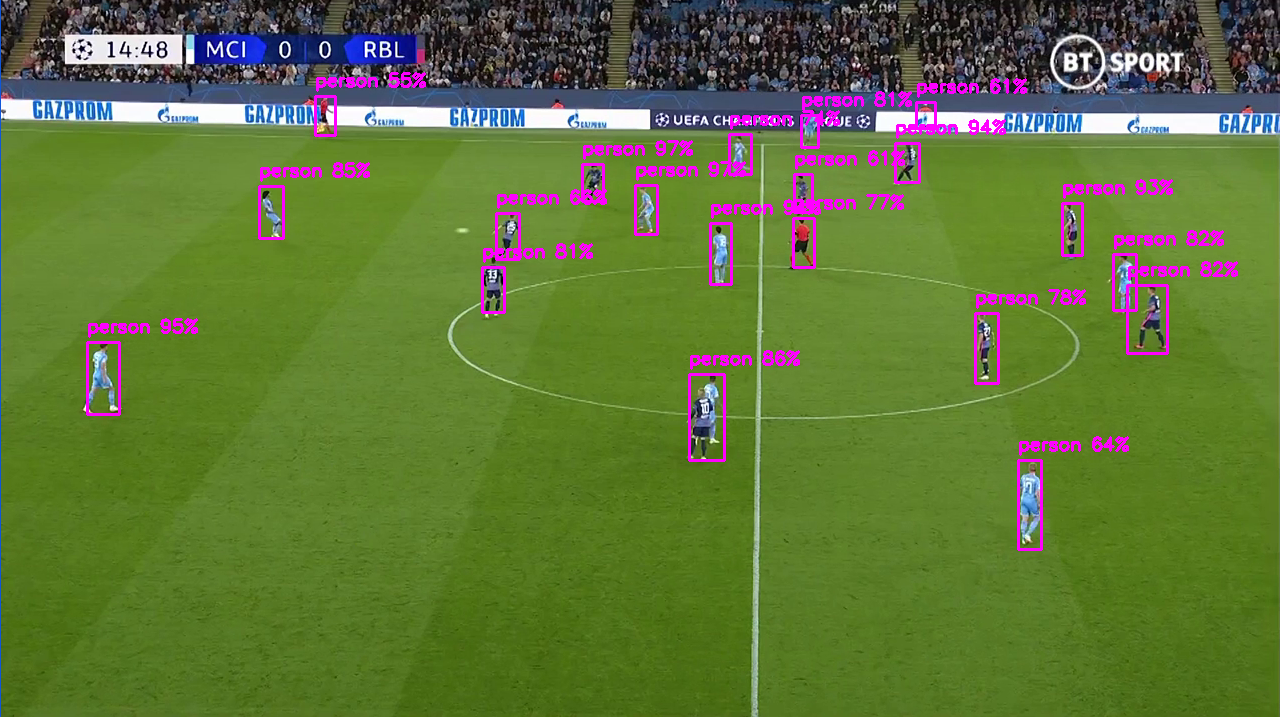
\includegraphics[keepaspectratio, width=\columnwidth]{first.png}
    \caption{caption}
    \label{img:1}
\end{figure}
\ref{img:1}
players are detected but ball is not (purple means that object recognition just ran). multiple players are detected in the same bounding box. refs are detected as well. one steward is also detected. streaming is stopped because ball is not found.
\begin{figure}[H]
    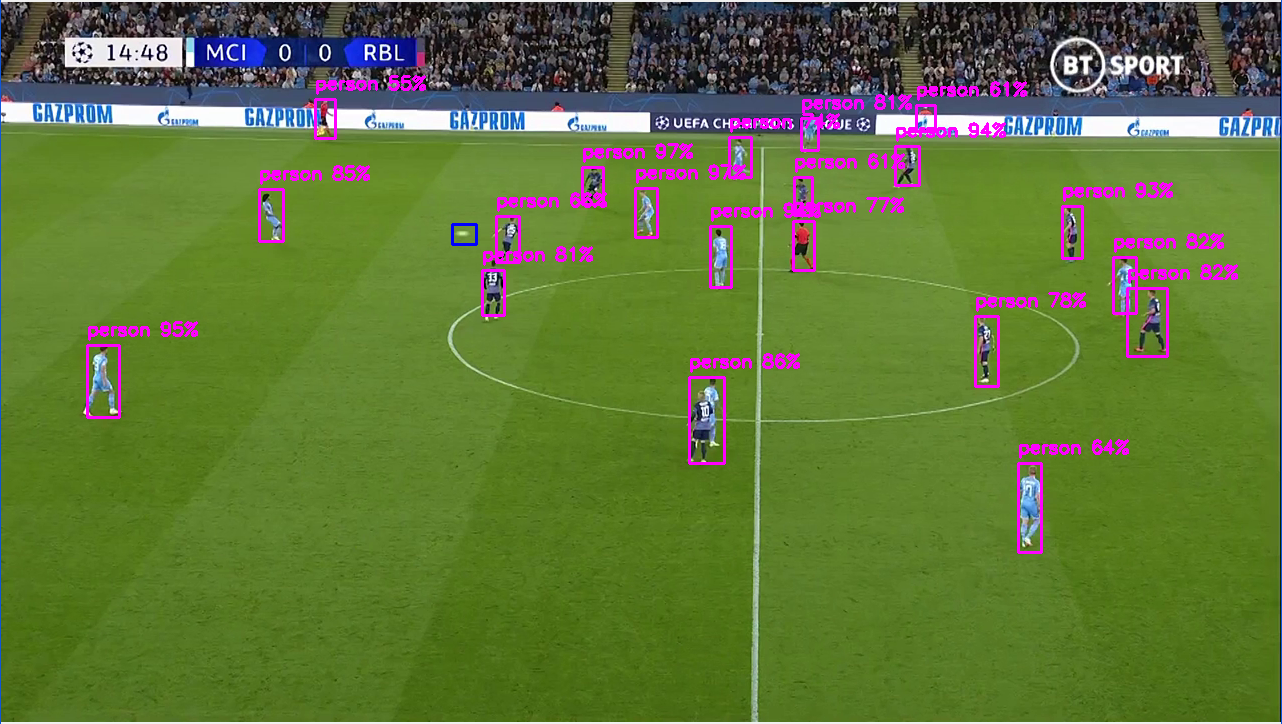
\includegraphics[keepaspectratio, width=\columnwidth]{Screenshot_2022-03-03_21-32-51.png}
    \caption{caption}
    \label{img:2}
\end{figure}
\ref{img:2} players bounding boxes in green means that it is tracking. manually labelling ball to continue stream.
\begin{figure}[H]
    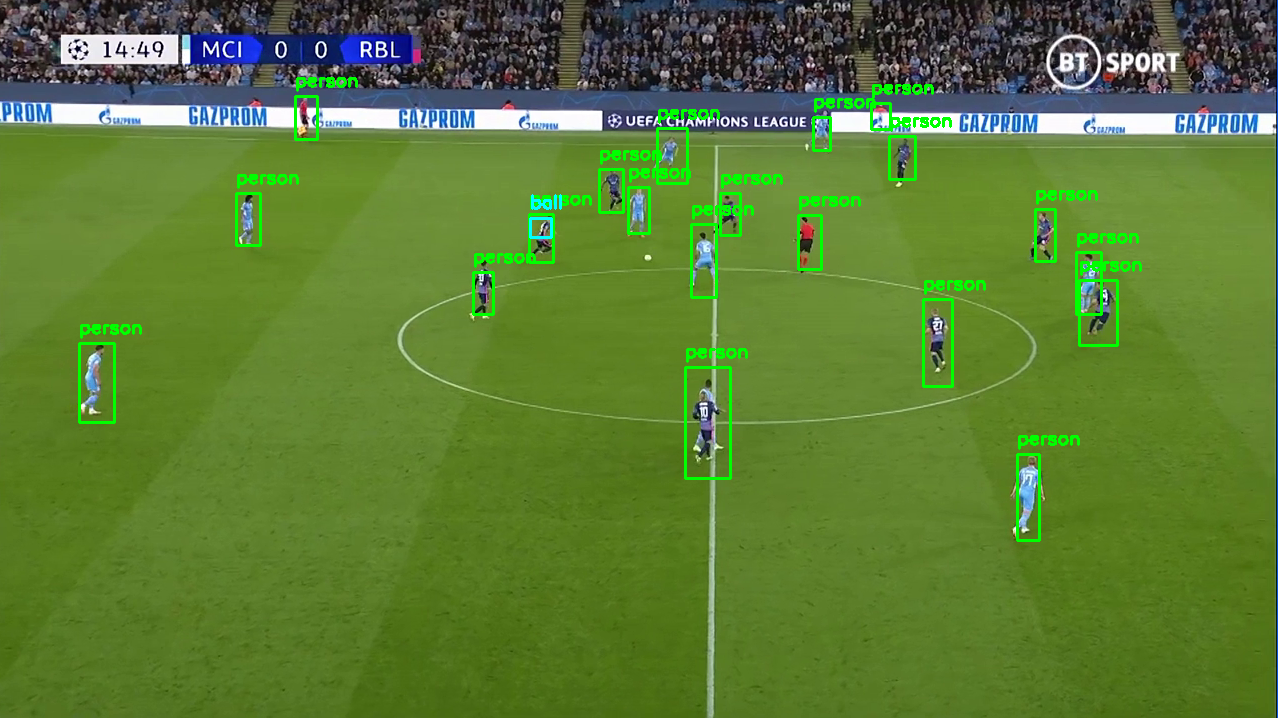
\includegraphics[keepaspectratio, width=\columnwidth]{Screenshot_2022-03-03_21-35-39.png}
    \caption{caption}
    \label{img:3}
\end{figure}
\ref{img:3} ball tracking is lost and tracks the numbers on the players back.
\begin{figure}[H]
    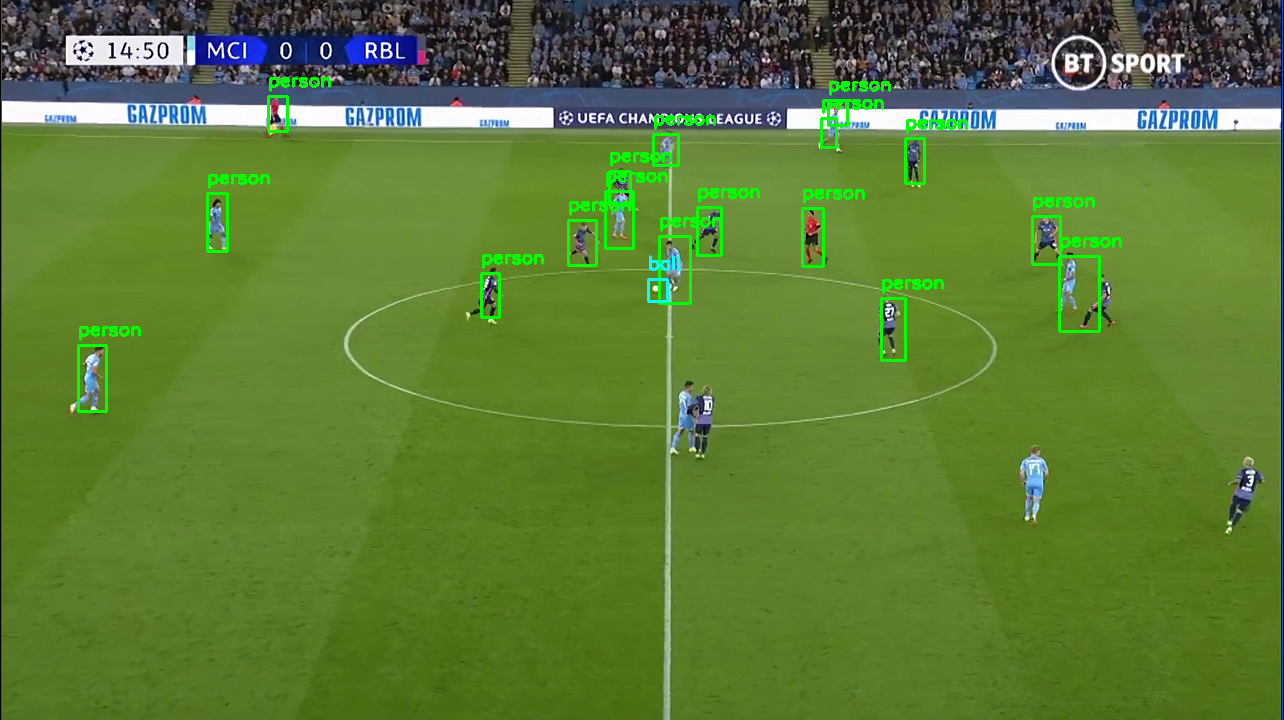
\includegraphics[keepaspectratio, width=\columnwidth]{Screenshot_2022-03-03_21-36-05.png}
    \caption{caption}
    \label{img:4}
\end{figure}
\ref{img:4} player tracking continues. new players appear on the screen but they are not
detected until 30frame period runs object detection again.
\begin{figure}[H]
    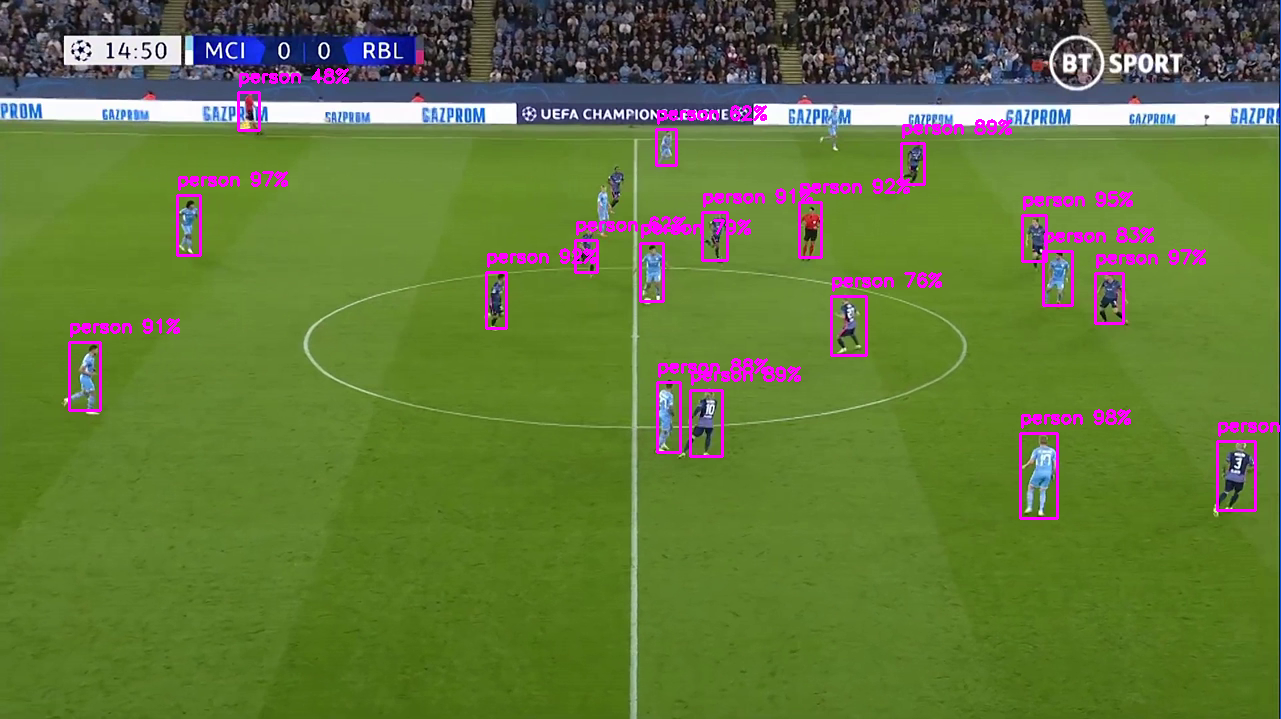
\includegraphics[keepaspectratio, width=\columnwidth]{Screenshot_2022-03-03_21-38-04.png}
    \caption{caption}
    \label{img:5}
\end{figure}
\ref{img:5} ball
tracking is lost again because of the pitch lines and player boots. some players previously detected are lost because of the backgroup from ads or pitch (not enough constract).
\begin{figure}[H]
    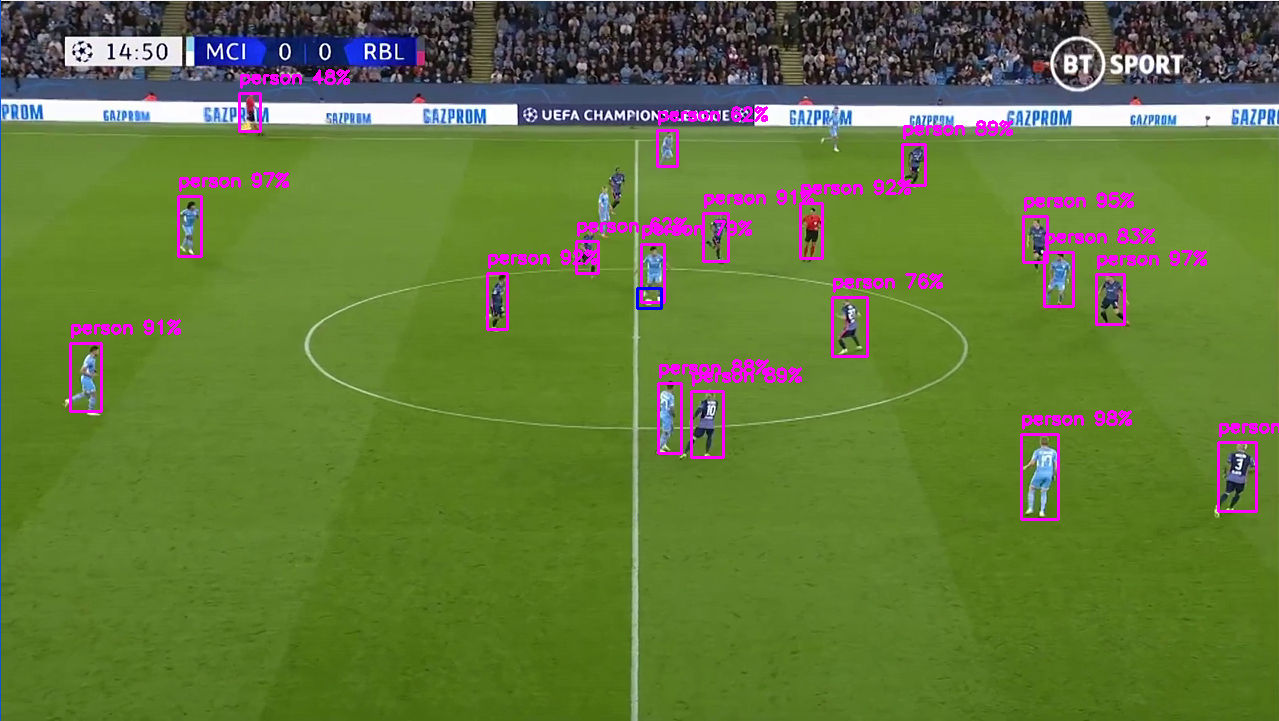
\includegraphics[keepaspectratio, width=\columnwidth]{Screenshot_2022-03-03_21-36-47.png}
    \caption{caption}
    \label{img:6}
\end{figure}
\ref{img:6} ball needs
to be labelled again to be tracked again.
\begin{figure}[H]
    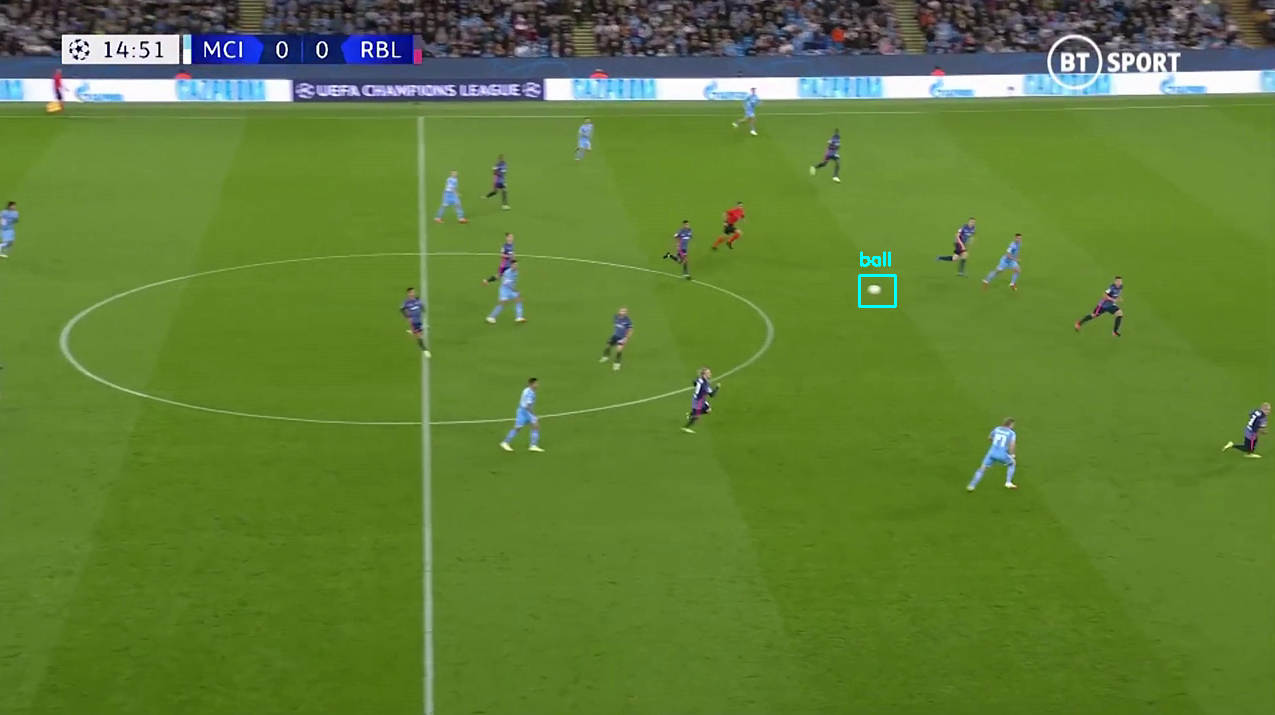
\includegraphics[keepaspectratio, width=\columnwidth]{Screenshot_2022-03-03_23-05-49.png}
    \caption{caption}
    \label{img:7}
\end{figure}
\ref{img:7} the object
detection is ran. all the human trackers are removed but the ball tracker. the ball tracker is not reset if the ball is still being tracked.
\begin{figure}[H]
    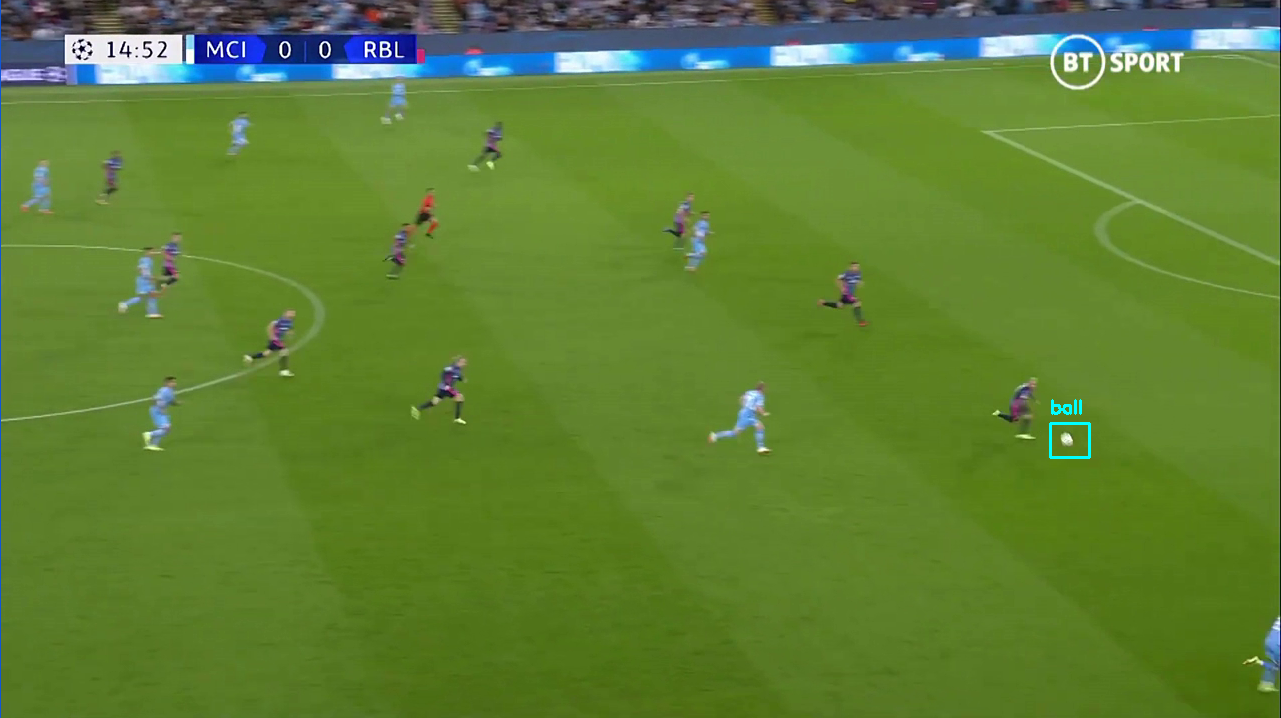
\includegraphics[keepaspectratio, width=\columnwidth]{Screenshot_2022-03-03_23-06-03.png}
    \caption{caption}
    \label{img:8}
\end{figure}
\ref{img:8} the
players tracker had to be reset again from the because the detected players moved out of the screen in the meantime. ball tracker continues to run, regardless.
\begin{figure}[H]
    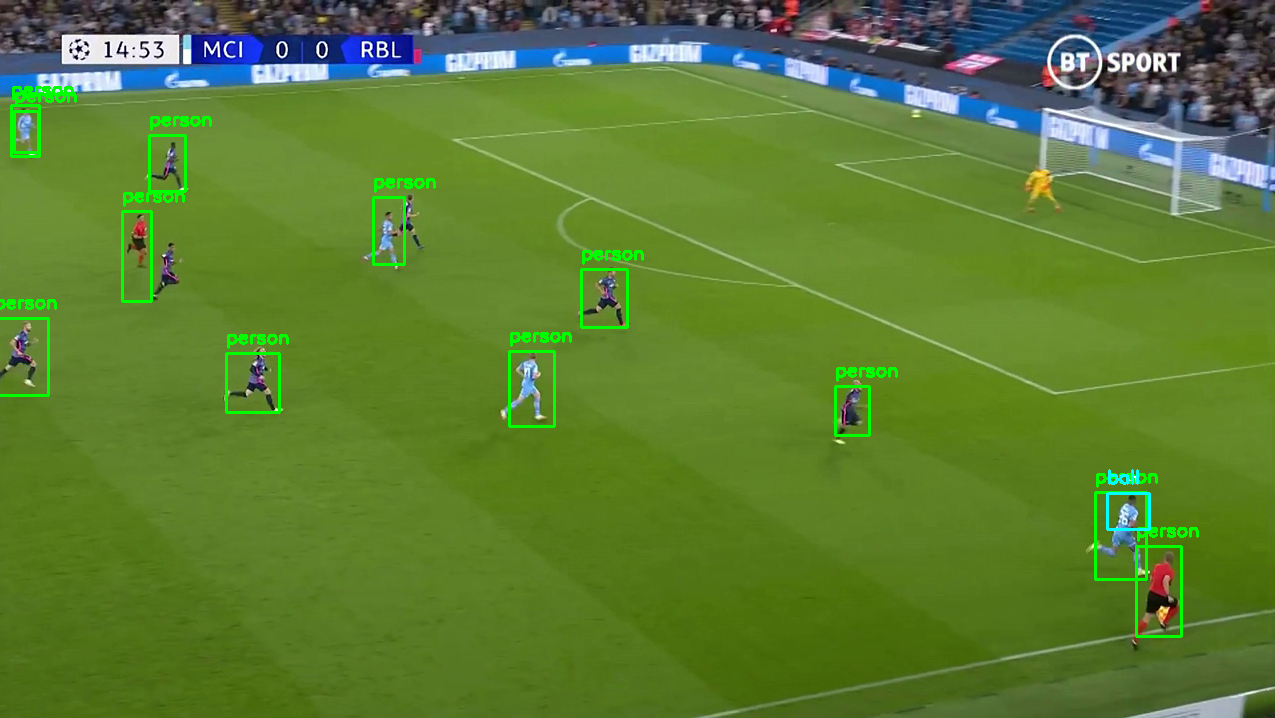
\includegraphics[keepaspectratio, width=\columnwidth]{Screenshot_2022-03-03_23-06-18.png}
    \caption{caption}
    \label{img:9}
\end{figure}
\ref{img:9} the ball
tracker is wrong again, by tracking the player's back number.
\begin{figure}[H]
    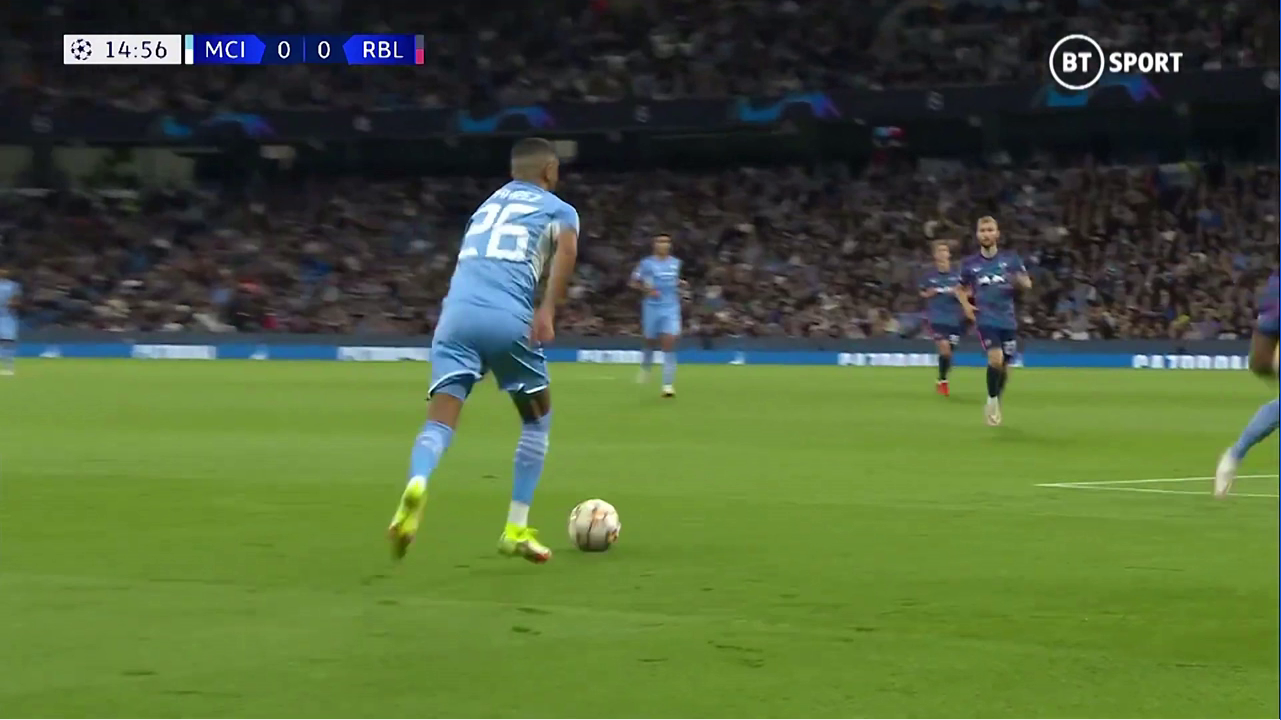
\includegraphics[keepaspectratio, width=\columnwidth]{Screenshot_2022-03-03_21-39-53.png}
    \caption{caption}
    \label{img:10}
\end{figure}
\ref{img:10} this is a
video segment imposed by the director. data cannot be collected. this is a short moment.
\begin{figure}[H]
    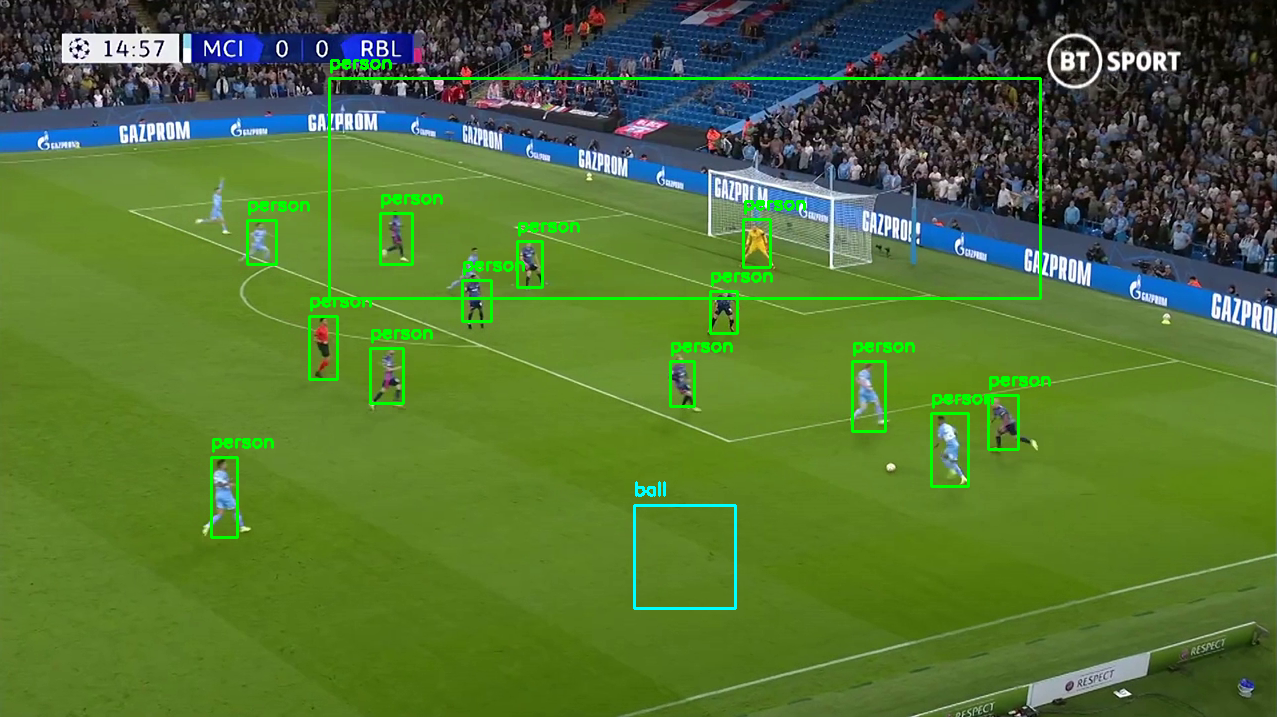
\includegraphics[keepaspectratio, width=\columnwidth]{Screenshot_2022-03-03_23-06-43.png}
    \caption{caption}
    \label{img:11}
\end{figure}
\ref{img:11} ball is
tracked from the since the label needs to be labelled for the stream to continue (needs to cut the scene). there is a bug, a human is recognised due to noise.
\begin{figure}[H]
    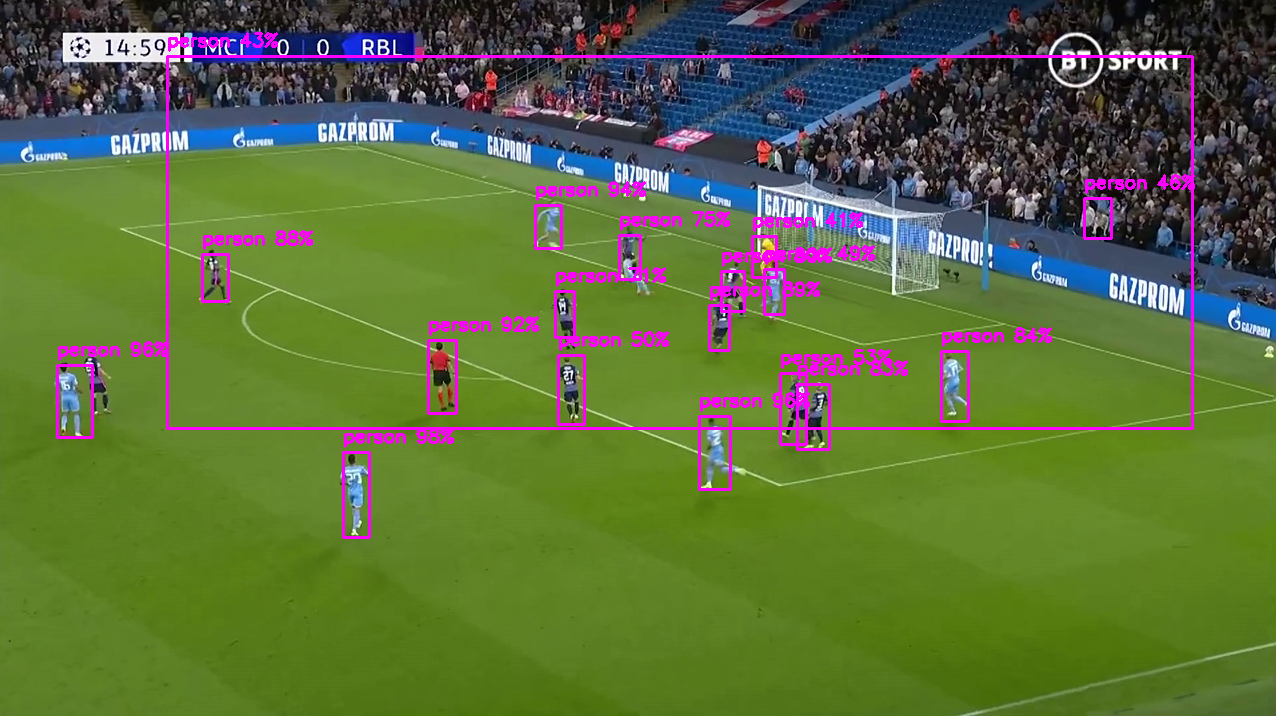
\includegraphics[keepaspectratio, width=\columnwidth]{Screenshot_2022-03-03_23-08-00.png}
    \caption{caption}
    \label{img:12}
\end{figure}
\ref{img:12} players
are detected again. the bug stil persists. a fan is recognised in the crowd. the ball is again not recognised.
\begin{figure}[H]
    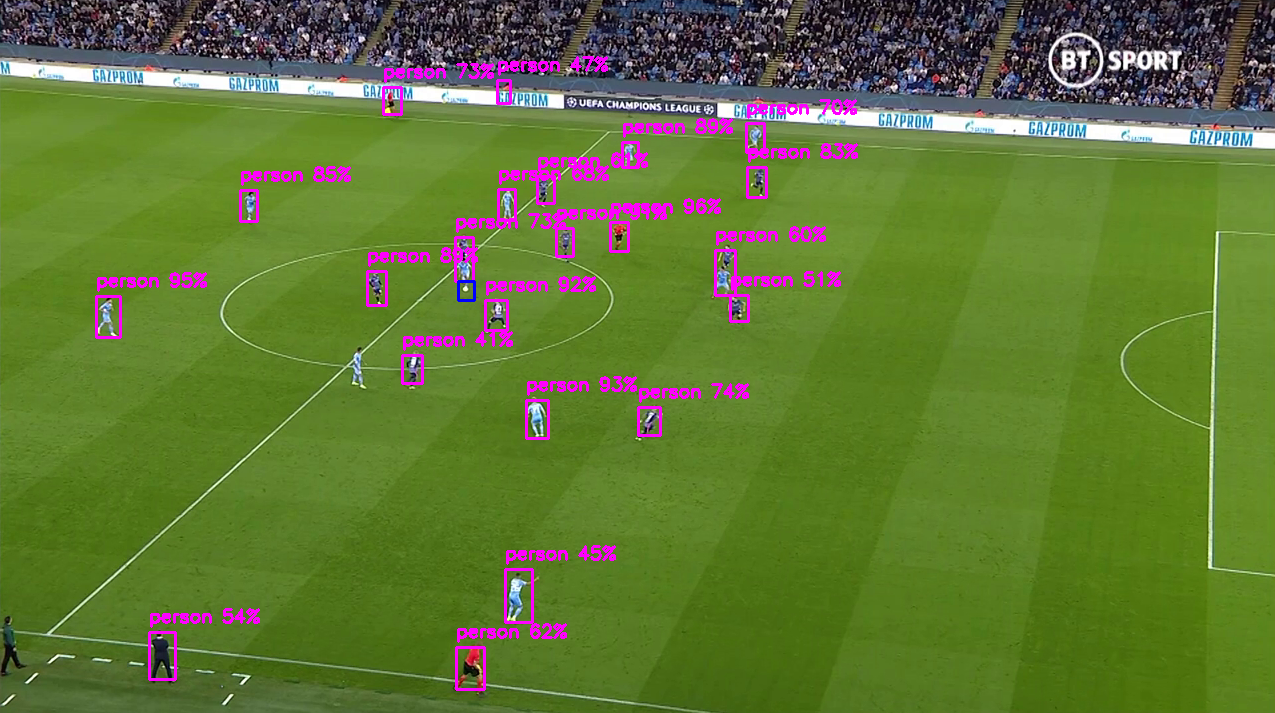
\includegraphics[keepaspectratio, width=\columnwidth]{Screenshot_2022-03-03_23-09-45.png}
    \caption{caption}
    \label{img:13}
\end{figure}
\ref{img:13} most
players are visible from this new perspective. The ball is not recognised.
\begin{figure}[H]
    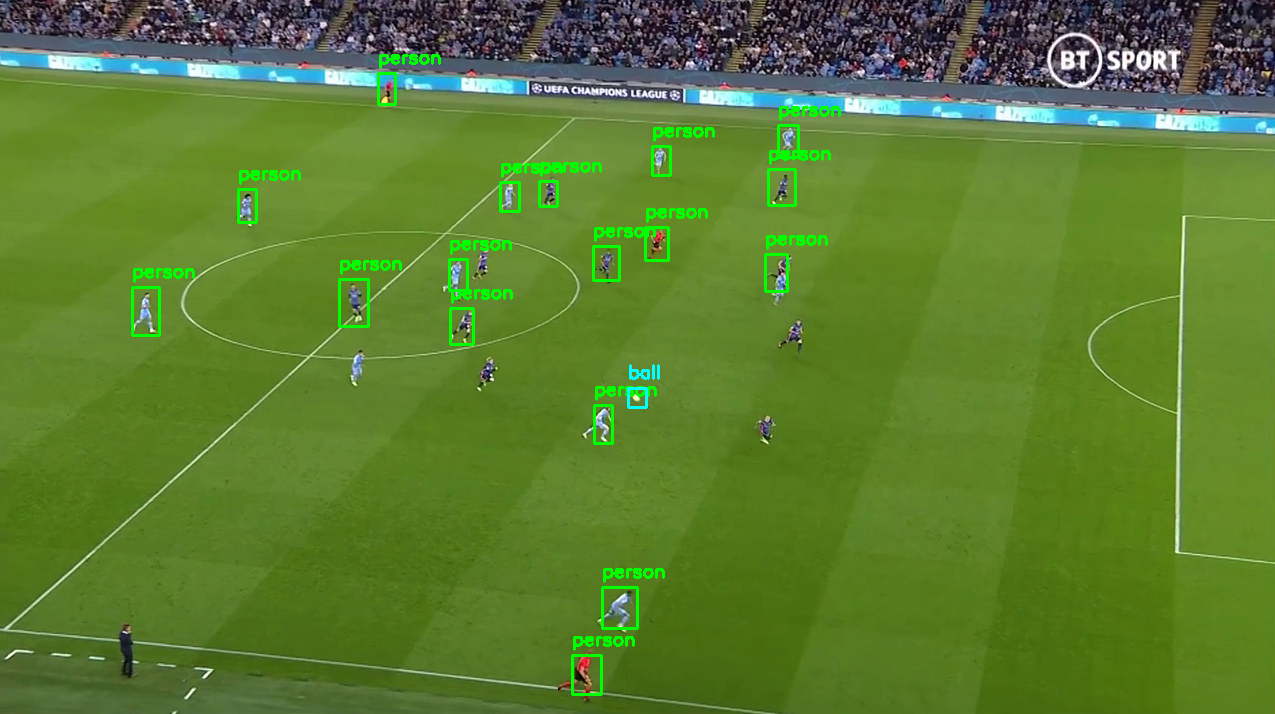
\includegraphics[keepaspectratio, width=\columnwidth]{Screenshot_2022-03-03_23-10-58.png}
    \caption{caption}
    \label{img:14}
\end{figure}
\ref{img:14} most of
the players are recognised from this perspective. The ball is visible and being tracked.
\begin{figure}[H]
    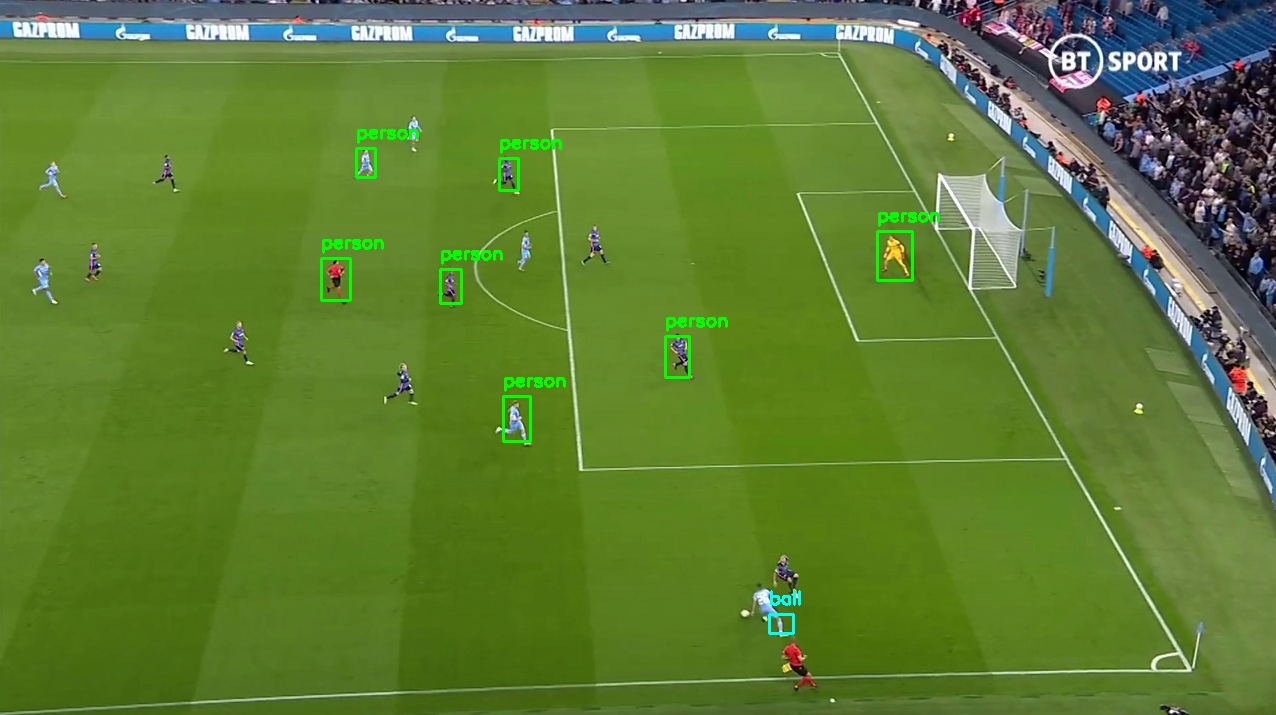
\includegraphics[keepaspectratio, width=\columnwidth]{Screenshot_2022-03-03_23-12-29.png}
    \caption{caption}
    \label{img:15}
\end{figure}
\ref{img:15} in this
frame few players were recognised because the camera view moved very suddendly (from the previous frame ) in betwee the object detection cycle. The ball tracker was lost and it is tracking the payer's leg instead.
\begin{figure}[H]
    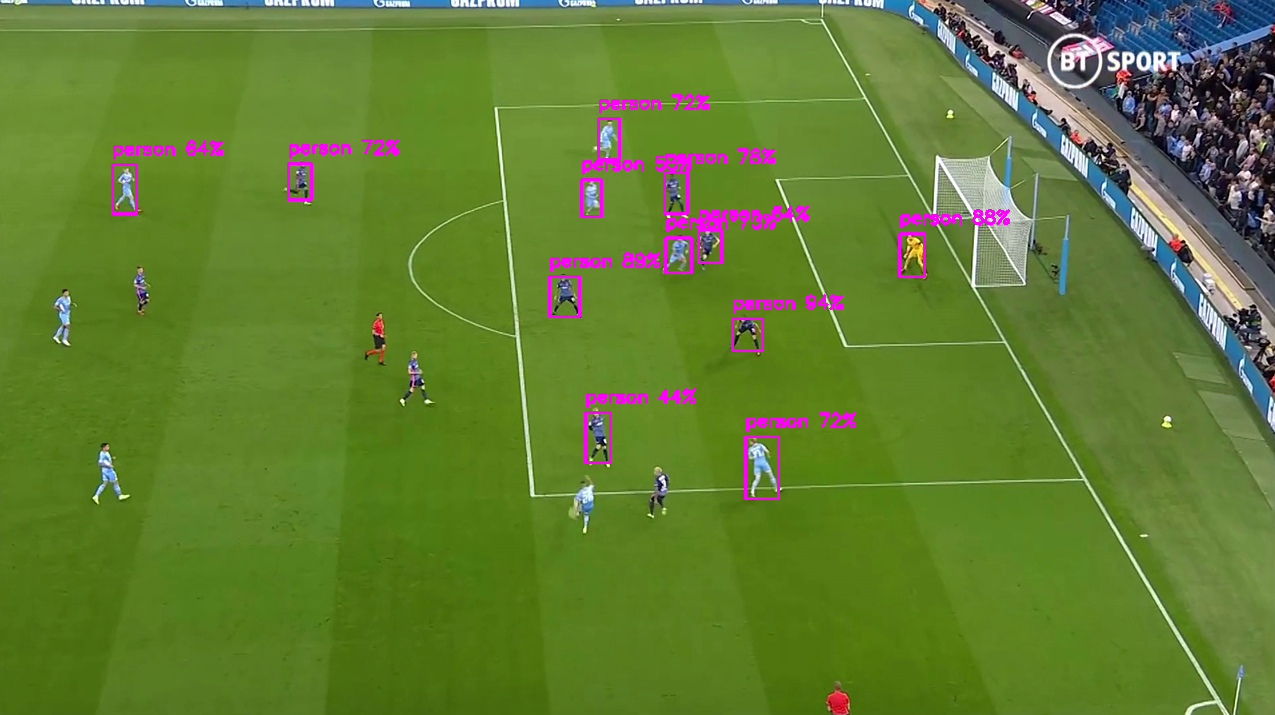
\includegraphics[keepaspectratio, width=\columnwidth]{Screenshot_2022-03-03_23-13-18.png}
    \caption{caption}
    \label{img:16}
\end{figure}
\ref{img:16} In this
frame most players are detected including all players inside the box which is the region of interest when a team is attacking. The ball tracker has lost the ball because the camera view is being blocked by the crossing player's leg. (sshot\textgreater{} pitch 3d modelling and camera automation)





\section{achievements and limits}

\subsection{achievements}


The most important achievement is the development of the foundations for a generic sports video data collection framework, as explained before. This was a challenging task since there are any other public full featured solution as this attempts to be. Although not all main features are not yet finished the project was planned to be a long term endeavour.
The image object detection and tracking algorithm is the most critical component in this system because without it data collection is not possible. This module may be changed but the algorithm will, a priori, remain the same as it fits the needs of other collective sports that are played with a ball.
The use of synthetic data is a novel and innovative way to approach the problem of creating a dataset for pitch recognition. The blender file has the realistic football pitch model but can also aggregate other sports by adding more scenes.
Another relevant achievement is the production of an end-to-end dataset generation framework that automates a set of cameras to simulate their normal activity. This framework is now mature and can already, as all the other modules, accommodate for other sports which is invaluable because it is now possible to create huge datasets for any sport.



\begin{itemize}
\item
creating recursively conditional machine learning model
\item
creating geometric framework to map objects from screen on pitch, and from pitch on to file
\end{itemize}


\subsection{limits}


\begin{itemize}
\item
  Human agent must verify and validate data collection
\item
  Human agent must manually segment video streams
\item
  Human agent must input match meta data
\item
  Human agent must supervise/calibrate video processing
\item
  Tracking broadcast is affected by zoom/replays and camera changes
\item
  human detection may contain more than 1 human non-consistent ball detection
\end{itemize}



\subsection{dissertation organisation sketch}


to fill in


\chapter{Background}


This chapter will delve into current research, projects and articles related to computer vision for sports' data extraction. The interest in this field is recent. However, there is already a comprehensive set of information sources necessary to evaluate the feasibility of developing a potential solution. Most of these sources lay out the scientific and technical principles applied in developing their successfully tested and solutions being assessed. Therefore, it is vital to have a deeper analysis and reflection on these principles to determine the most appropriate approach for this Project. The review aims to gather the knowledge required to develop and evaluate this Project's solution successfully.


\section{Basketball video analysis}


The ``Open Source Sports Video Analysis using Machine Learning'' article \cite{stephan} is an excellent article that lays out a real-world application of the theory behind automated sports analytics video extraction. It serves as a complete description of the ``basketballVideoAnalysis'' open-source project \cite{stephan_code} that has the goal of tracking players, objects and actions for allowing the analysis of basketball match recordings. This article is a good starting point for this review because Stephan does a good job explaining complex theories in more straightforward terms and referencing other authoritative resources that must be considered to further expand on if anyone is interested in developing a similar solution. The Project used the ``Player tracking and analysis of basketball plays'' \cite{baskettrack} research as the blueprint for its planning and development. Stephan also suggests that this algorithm can be adapted for other collective sports. The article \cite{stephan} goes on to describe that the ``basketballVideoAnalysis'' project can track the match by executing a machine learning and image processing pipeline. This pipeline consists of basketball court detection, tracking humans inside the court, and mapping their movements to their position relative to the court.


Court detection is critical in this system because there is no reference needed to position objects (human bodies and ball) and filter out the noise (all remaining objects outside the court). The surface detection, in this article, is a pure image processing algorithm composed of naive OpenCV \cite{opencv} functionalities such as HSV conversion, Hue range filtering, Bitwise-AND masking, Canny edge detection and Hough Transformation. These functionalities' combination filters the input's noise out and increases the machine learning features' intensity.


The following step is to detect the people in the court, which is essential because it extracts the segmented image containing the person's to be used for further measures such as player identification, player tracking, homographic mapping, pose estimation and action recognition. The people detection is undertaken using robust common object detection models and training them against existing image curated datasets, for instance, the COCO image dataset \cite{cocodataset}.


The article points out how identifying players can be challenging by quoting an excerpt from ``Learning to Track and Identify Players from Broadcast Sports Videos'' \cite{learn_track_id} that describes the technical and logistical obstacles associated with this task.


The last step in Stephan's Project is to map the current camera view to a reference map to accurately determine where objects (including people) are in the field. In this operation, the OpenCV \cite{opencv} ``findHomography'' takes the original image points and the reference map coordinates to transform and map the original image onto the reference map.


Despite this article being a helpful starting point for research, it lacks academic research and implementation rigour. This is evident by the absence of any meaningful citation.


\section{Player tracking and analysis of basketball plays}

This project \cite{baskettrack} focuses on creating automated player detection and tracking system using the Matlab programming language. The basketball court detection in this Project is accomplished solely by using image processing techniques such as converting the colour format, eroding and dilating the image before applying the canny edge detector, and Hough transform. This process of court detecting appears to be very efficient as it is not a complex algorithm. This is highly effective for basketball, but it might not work as well in a football match. A football pitch is bigger than in basketball, and the camera is zoomed in to focus on a particular pitch zone. This fact, in football, forces a possible solution to find a way of augmenting the possible location the camera is focused on. The same pipeline, created by ``Player tracking and analysis of basketball plays'' research, should be used in our Project, but it needs to be complemented by machine learning and augmentation because basketball recordings have a significantly bigger percentage on the court \cite{baskettrack}.


The player detection is applied inside the court detection region by executing the OpenCV's \cite{opencv} HOG detector (histogram of oriented gradients) to create bounding boxes around players. This detector focuses on measuring the gradients' orientation on image's regions to detect patterns that recognise human bodies. This technique needs to be adjusted, during the testing stage, by adjusting the detection threshold adjusted to filter out false positives or just general noise. The approach is generally very effective unless two or more players are crossing in the camera view field. The authors decided to run the OpenCV's BGR detector inside the HOG detector bounding box since teams usually have different colours. This player detection algorithm is simple and accomplishes most of its purposes; however, it does not address players from the same team crossing the camera view. This event is very common in collective sports and should be a high requirement due to its occurrence frequency. An algorithm that uses human pose posture detection or other machine learning algorithms should effectively mitigate this important issue.


The team, following the implementation of the player detection algorithm, moved to work on player tracking. After some development, they identified four common tracking scenarios:
\begin{enumerate}
\item Player detected in consecutive frames: player was detected by HOG and BGR detectors;
\item Neighbourhood estimate: player was only detected by the BGR detector in the neighbourhood of the previous HOG detection;
\item Players added to frame;
\item Players removed from the frame.
\end{enumerate}
The first two scenarios are relatively easy to handle by applying the minimum distance correlator that calculates the most likely last position according to the current position. The last two cases are more complicated than the previous ones, and the Project did not mitigate them. Some of the reasons were the tracking of false positives (players on the bench just next to the court) and the camera jitter, which can affect the court view and the players' position on the camera view itself. The project \cite{baskettrack} was not successful in this step perhaps because it did not try to create an image recognition system that would train to learn the players' visual features (including the shirt number), as well as creating a machine-learning algorithm to augment the possible movement of players off the screen considering the last and first (when it reappears) position/speed.


Finally, the tracking data needs to be mapped to a model court by running a homography matrix. This matrix is generated through an affine transformation relative to the camera view towards the basketball court. This process is effective because the court and players' position is already known, and the matrix operation is very efficient in a numerical computing programming language like Matlab.



\section{Learning to track and identify players from broadcast sports videos}


The research analyses how to pre-process video and detect, identify and track players from a camera recording and map them to a referential map. It is a very extensive explanation that introduces video processing and player identification. Despite having many relevant requirements, the researchers decided not to have action recognition \cite{learn_track_id}.

Video pre-processing is composed of two steps: video segmentation and then ``play-by-play'' data processing. This pre-processing combination captures and aggregates relevant data used for data augmentation on the next pipeline layers. The video segmentation takes full recordings (sequence of different camera/video shots such as replays, ads, focus zoom), trains a complex model that uses Hidden Markov Model, Gaussian Mixture Model and the Viterbi algorithm to predict the segments and which type they are based on the colour distribution. The ``play-to-play'' data is a sequential, freely available online stream that tracks the most important match events. This type f data is very important in the player identification and could be very useful for action recognition if it was a requirement \cite{learn_track_id}.

The player tracking detects the players inside the court by running a Deformable Part Model, which can identify most players, but it has mediocre precision since it detects people in the audience and the referees, and it does not detect players obstructed in the camera angle. Before training a Linear Logistic Classifier, the false positives (audience and referee) are removed by applying team colour (since all teammates have the same colour but are different from the opposition or referee). The player tracking follows the bounding boxes' centre points from the player detections and tries to predict the following position based on the Euclidean distances of previous positions by executing a linear-Gaussian transition model. The precision of this tracking technique has a very high precision since it only tracks single points (simple and minimal algorithm) and drops sparse tracking or view borders signals \cite{learn_track_id}.
The player identification is an exciting and unique challenge set by the researchers. It poses serious questions about how its efficiency due to:

\begin{itemize}
\item same team players have the same kits;
\item recording with resolution too low for facial recognition;
\item some players might have similar body characteristics, hairstyles, or boots;
\item shirt numbers and names are deformed due to constant posture changes \cite{learn_track_id};
\end{itemize}


The solution for player identification focuses on learning players' visual features/characteristics, dismissing trying to identify players' faces \cite{learn_track_id}. The input to identify these features are:

\begin{itemize}
\item Maximal extremal regions (MSRE);
\item Scale-invariant feature transform (SIFT);
\item RGB colour histograms;
\end{itemize}


These image processing features and the bounding box image segment are the input for a complex algorithm that continuously learns each player's visual characteristics and identifies them \cite{learn_track_id}.
The homography transformation is calculated by representing the referential basketball court as a set of points. The Canny Edge detector processes the image with a certain threshold to remove noise and drop nonlinear or well-rounded lines until only the court shape is visible. Following this process constructs the homography matrix by incrementally detecting the corresponding points (nearest points) until it converges in at most five iterations, at most \cite{learn_track_id}.

\section{Multi-Person 3D Pose Estimation and Tracking in Sports}






This Project aims to process multiview recordings, detect and correct players' 2D pose estimations, associate the 2D poses into a 3D pose and track the 3D poses. Pose estimation is very important because it has the potential to allow for action recognition. The researchers consider this Project as the pioneering in full 3D pose estimation tracking for sports. The Project used advanced research from previous work on 3D pose estimation and multiview video recording to develop a very optimised process to capture this kind of data for Football \cite{cvpr_2019}. The algorithm follows these general steps:

\begin{itemize}
\item 2D pose estimation
\item 2D pose error correction
\item 2D pose multiview association to 3D pose
\item 3D skeleton tracking
\end{itemize}

The Project uses a CNN-based model to train in the ``Surreal'' synthetic dataset \cite{surreal} and subsequently estimate the 2D pose of players.
The initial pose estimation is prone to errors due to low-quality image, view cut, and multi-person fusion, so the pose error correction is vital to correct these common errors. The researchers decided on a per-frame pose correction solution rather than a temporal filtering and tracking algorithm because its performance is significantly better \cite{cvpr_2019}.
The next step is to associate the two 2D pose estimations from a single frame by running a greedy algorithm that measures the pair of corresponding points. Once this correspondence is asserted, then the 3D joint locations can be calculated. Once the 3D joint location is calculated, then it can be constructed and mapped to the 3D court model \cite{cvpr_2019}.
The final step is to sequentially track the resultant 3D pose models around the pitch what is very impressive because it is a full 3D model of a football match \cite{cvpr_2019}.






\section{Soccer: Who Has The Ball? Generating Visual Analytics and Player Statistics}


This Project is a solution that generates visual analytics and player statistics from football recordings. This is an important paper because it aims to recognise actions using deep neural networks from single frames in football matches. The paper also describes the architecture of the different deep neural networks used for, as mentioned before, for the action recognition but also the player location detection \cite{cvpr_2018}.




The first part of this algorithm is to locate, track the player and detect the team. The location is done by running the YOLO algorithm, which predicts the bounding boxes containing every player on the camera view. These bounding boxes are then tracked during the consecutive by another model also using the YOLO algorithm. This tracking phase is then finished by running a Histogram Matching algorithm inside the bounding box to identify the player's team. The Histogram Matching algorithm was chosen because it is fast at detecting different colours (teams' kits are always different), and the task is relatively simple since the player is inside a small region \cite{cvpr_2018}.






The last step is to identify if the player is "in control of the ball" or not and then augment data from this information. The researchers created an image dataset with images (segments of images, zoomed into the player) of individual football players and then classified the images with either "player with the ball" or "player without the ball" classes. This part of the algorithm then took the synchronised sequence of images and predicted data to keep track of the player holding the ball. This information is relevant because it is possible to deduce with spatio-temporal precision the possession of the ball by a team since it is the sequence of players "having the ball". The spatio-temporal event between players of the same team "having the ball" is a pass (where the start and end location is also known) otherwise is an opposition "ball recovery". Generating an automatic model of possession is precious because it is the most frequent activity the football teams engages in, and it is the most relevant way football domain experts take into consideration when analysing football \cite{cvpr_2018}.




\section{Conclusion}




This background research was vital to understanding the foundations of the current solutions in the field. Based on the current acquired information, this Project's goal is possibly accomplished by decomposing the problem into a pipeline composed by:

\begin{itemize}
\item Court detection;
\item Object detection;
\item Team identification;
\item Object tracking;
\item Player identification;
\item Homographic mapping of objects.
\end{itemize}


The important idea to remember is that there is already robust technologies and methodologies necessary for this solution. This knowledge gained should provide a solid foundation to develop a proper implementation of a similar solution.



\chapter{Implementation}







To add to methods section



\listofalgorithms


pseudocode for main code





\begin{algorithm}
\begin{algorithmic}

\caption{findObjects procedure}\label{alg:findObjects}
\Require \\
    $frame: OpenCVFrame$ \\
    $model: YoloModel$ \\
    $c: ObjectConfidenceThreshold$ \\
    $b: BallConfidenceThreshold$
\Ensure \\
    $objs: ObjectsBoxes$ \\
    $ball: BallBox$

\State $$

\State $predictions \gets model.predict(frame)$
\State $objs$ \gets \emptyset

\For {$prediction \in predictions$}
    \If {$prediction \Is person$ \And $c < conf$}
        \State $objs.append(prediction)$
    \EndIf
    \State
    \If {$prediction \Is ball$ \And $b < conf$}
        \State $ball \gets prediction$
    \EndIf
    \State
\EndFor
\State
\State \Return $objs, ball$

\end{algorithmic}
\end{algorithm}





\begin{algorithm}
\begin{algorithmic}

\caption{main}\label{alg:cap}

\Require \\
    $frame: OpenCVFrame$ \\
    $ballTracker: Tracker$ \\
    $objTracker: Tracker$

\State $$

\State $frameCount \gets 0$


\For { $frame \in video$ }
    \If { $frameCount \bmod 30 = 0$ }
        \State $performDetection \gets true$
    \Else
        \State $performDetection \gets false$
    \EndIf


    \If { $performDetection$ }
        \State $objs, ball \gets findObjects(frame)$

        \If {$length(objs) > 0$ }
            \For { $o \in objs$ }
                \State $objTracker.add(o)$
            \EndFor

            \State $frameCount \gets frameCount + 1$
        \EndIf

        \If { $ball$ }
            \State $ballTracker.init(ball)$
        \Else
            \State $ball \gets labelBall(frame)$
            \State $ballTracker \gets Tracker(ball)$
        \EndIf

    \Else

        \State $isTracking, boxes \gets objTracker.update(frame)$

        \If { $isTracking$ }
            \State $frameCount \gets frameCount + 1$
        \Else
            \State $frameCount \gets 0$
        \EndIf

        \State $isTracking, box \gets ballTracker.update(frame)$

        \If {$\Not isTracking$}
            \State $ball \gets labelBall(frame)$
            \State $ballTracker \gets Tracker(ball)$
        \EndIf

    \EndIf

\EndFor


\end{algorithmic}
\end{algorithm}


\item
  pseudocode for 3-d modelling data set generation
\end{itemize}


\begin{algorithm}
\begin{algorithmic}


\caption{encodeData}\label{alg:cap}

\Procedure{encode\_vector}{$vector$}
    \Return $tuple($
        \State \indent $vector.x,$
        \State \indent $vector.y,$
        \State \indent $vector.z$
    \State $)$
\EndProcedure

\Procedure{encode\_vector\_list}{$list$}
    \Return $reduce($
        \State \indent $\lambda rest\_data, last: rest\_data + encode\_vector(last),$
        \State \indent $list,$
        \State \indent $[]$ \Comment{$initial value$}
    \State $)$
\EndProcedure


\Procedure{corner\_vecs\_pitch\_vecs}{$pitch\_vectors$}
    \State $corner\_vectors \gets \emptyset$
    \State $p\_corners \gets \emptyset$
    \For {$i \in pitch\_vectors$}
        \If {$i \in [0, 9, 29, 38]$}
            \State $corner\_vectors.append(pitch\_vectors[i])$
        \Else
            \State $p\_corners.append(pitch\_vectors[i])$
        \EndIf
    \EndFor
    \State
    \Return $($
        \State \indent $corner\_vectors,$
        \State \indent $p\_corners$
    \State $)$
\EndProcedure

\State

\Procedure{encodeData}{$data$}
    \State $origin, framesVectors, pitchVectors \gets data$

    \State

    \State $encodedOrigin \gets encode\_vector(origin)$

    \State $encodedFramesVectors \gets encode\_vector\_list(framesVectors)$

    \State $corner\_vectors, pitch\_vectors \gets corner\_vecs\_pitch\_vecs(pitch\_vectors)$

    \State $encodedCornerVectors \gets encode\_vector\_list(pitchVectors)$

    \State $encodedPitchVectors \gets encode\_vector\_list(pitchVectors)$

    \Return $($
        \State \indent $encodedOrigin +$
        \State \indent $encodedFramesVectors +$
        \State \indent $encodedCornerVectors +$
        \State \indent $encodedPitchVectors$
    \State $)$
\EndProcedure

\end{algorithmic}
\end{algorithm}



\begin{algorithm}
\begin{algorithmic}


\caption{An algorithm with caption}\label{alg:cap}

\State

\Procedure{getData}{$camera$}

    \State $camOriginVector \gets camera.matrix.translation()$

    \State $framesVectors \gets camOrigin.frames()$

    \State $pitchVectors \gets \emptyset$

    \For {$marker \in blender.collection("pitch markers")$}
        \State $pitchVectors.append(marker)$
    \EndFor

    \Return $origin, framesVectors, pitchVectors$
\EndProcedure

\State

\For {$camera \in cameras$}
    \State $fileName \gets blender.renderImage(camera)$

    \State $data \gets getData(camera)$

    \State $encodedData \gets encodeData(data)$

    \State $writeToCsv(fileName, encodedData)$

    \State $camera.changeAngle()$
\EndFor

\State

\end{algorithmic}
\end{algorithm}


\begin{itemize}
\item
  machine learning model and algorithm
\end{itemize}


\begin{algorithm}
\begin{algorithmic}


\caption{An algorithm with caption}\label{alg:cap}
\Require \\
    data: ModelData \\
    params: ModelParameters \\
    w: IMG\_WIDTH \\
    h: IMG\_HEIGHT

\State $

\State $outputSize \gets params.outputSize$


\State $secondaryInputLen \gets params.secondaryInputLen$


\State $convolutionLayers \gets [$
    \State \indent $Input(w, h),$
    \State \indent $Convolution2D(),$
    \State \indent $flatten()$
\State $]$


\State $output \gets Output(outputSize)$


\If {$secondaryInputLen > 0$ }

    \State $secondaryInput \gets [$
        \State \indent $Input(secondaryInputLen)$
    \State $]$

    \State $model \gets Model($
        \State \indent $input \gets concatenate($
            \State \indent \indent $secondaryInput,$
            \State \indent \indent $convolutionLayers$
            \State \indent $),$
            \State \indent $outputs \gets output$
    \State $)$

\Else

    \State $model \gets Model($
        \State \indent $input \gets convolutionLayers,$
        \State \indent $outputs \gets output$
    \State $)$

\EndIf

\State $compileModel(model, data, params)$


\end{algorithmic}
\end{algorithm}



\begin{algorithm}
\begin{algorithmic}


\caption{An algorithm with caption}\label{alg:cap}

\Require \\
    data: ModelData \\
    params: ModelParameters

\State $

\State $trainModel( data, ($
    \State \indent $model \gets "camOriginVec",$
    \State \indent $outputSize \gets 3,$
    \State \indent $secondaryInputLen \gets 0,$
    \State \indent $\ldots params$ \Comment{$rest$}
\State $) )$

\State $

\State $trainModel( data, ($
    \State \indent $model \gets "frameVectors",$
    \State \indent $outputSize \gets 12,$
    \State \indent $secondaryInputLen \gets 3,$
    \State \indent $\ldots params$ \Comment{$rest$}
\State $) )$

\State

\State $trainModel( data, ($
    \State \indent $model \gets "pitchCornerVecs",$
    \State \indent $outputSize \gets 8,$
    \State \indent $secondaryInputLen \gets 15,$
    \State \indent $\ldots params$ \Comment{$rest$}
\State $) )$

\State

\State $trainModel( data, ($
    \State \indent $model \gets "pitchVectors",$
    \State \indent $outputSize \gets 70,$
    \State \indent $secondaryInputLen \gets 23,$
    \State \indent $\ldots params$ \Comment{$rest$}
\State $) )$

\State


\end{algorithmic}
\end{algorithm}


\begin{algorithm}
\begin{algorithmic}


\caption{An algorithm with caption}\label{alg:cap}


\State

\Procedure{getModelPred}{$modelNames, X$}

    \If {$modelNames = \emptyset $}
        \State
        \Return $X$
    \EndIf

    \State $curr\_model \gets modelNames[0]$
    \State $rest\_models \gets modelNames[1:]$
    \State $pred \gets curr\_model.predict($
            \State \indent $frame,$
            \State \indent $X$
    \State $)$


    \Return $getModelPred($
        \State \indent $rest\_models,$
        \State \indent $X + pred$
    \State $)$


\EndProcedure

\State
\State


\Procedure{getFramePrediction}{$frame$}
    \State
    \Return $getModelPred([$
        \State \indent $"camOriginVectors",$
        \State \indent $"frameVectors",$
        \State \indent $"pitchCornerVectors",$
        \State \indent $"pitchVectors"$
        \State \indent $],$
        \State \indent \emptyset
        \State
    \State $)$

\EndProcedure


\end{algorithmic}
\end{algorithm}




\begin{itemize}
\item
  geometry reconstruction algorithm
\end{itemize}


\begin{algorithm}
\begin{algorithmic}


\caption{decodeData}\label{alg:cap}


\Procedure{dec\_vec}{$list$}
    \Return $tuple($
        \State \indent $list[0],$
        \State \indent $list[1],$
        \State \indent $list[2]$
    \State $)$
\EndProcedure

\Procedure{dec\_list}{$data, decode\_fun, unit\_length$}
    \State
    $data\_len = length(data)$
    \If {$data\_len = 0$}
        \Return $data$
    \EndIf

    \State $rest\_of\_data \gets data[:data\_len - unit\_length]$

    \State $data\_to\_decode \gets data[data\_len - unit\_length:]$
    \State $decoded \gets decode\_fun(data\_to\_decode)$

    \Return $dec\_list($
            \State \indent $rest\_of\_data,$
            \State \indent $decode\_fun,$
            \State \indent $unit\_length$
    \State $) + [decoded]$
\EndProcedure


\Procedure{decode\_vector\_list}{$lst, length$}
    \Return $dec\_list($
        \State \indent $lst,$
        \State \indent $\lambda data: dec\_vec(data, length),$
        \State \indent $length$
    \State $)$
\EndProcedure


\Procedure{decode\_camera\_data}{$enc\_data$}


    \State $($
    \State \indent $origin\_decoded, frames\_vectors\_data, corner\_vectors\_data, pitch\_vectors\_data$
    \State $) \gets get\_data\_ranges(enc\_data)$

    \State $origin\_decoded \gets dec\_vec(origin\_enc\_data)$

    \State $frames\_vectors\_decoded \gets decode\_vector\_list(frames\_vectors\_data, 3)$

    \State $corner\_vectors\_decoded \gets decode\_vector\_list(corner\_vectors\_data, 3)$

    \State $pitch\_vectors\_decoded \gets decode\_vector\_list(pitch\_vectors\_data, 3)$

    \State $pitch\_vectors\_decoded \gets merge($

    \Return $($
        \State \indent $origin\_decoded,$
        \State \indent $frames\_vectors\_decoded,$
        \State \indent $pitch\_vectors\_decoded$
    \State $)$

\EndProcedure



\end{algorithmic}
\end{algorithm}




\section{video processing}

- machine learning humans and ball recognition
- object traking


\section{3d modelling and dataset generation}


text




\begin{figure}[H]
    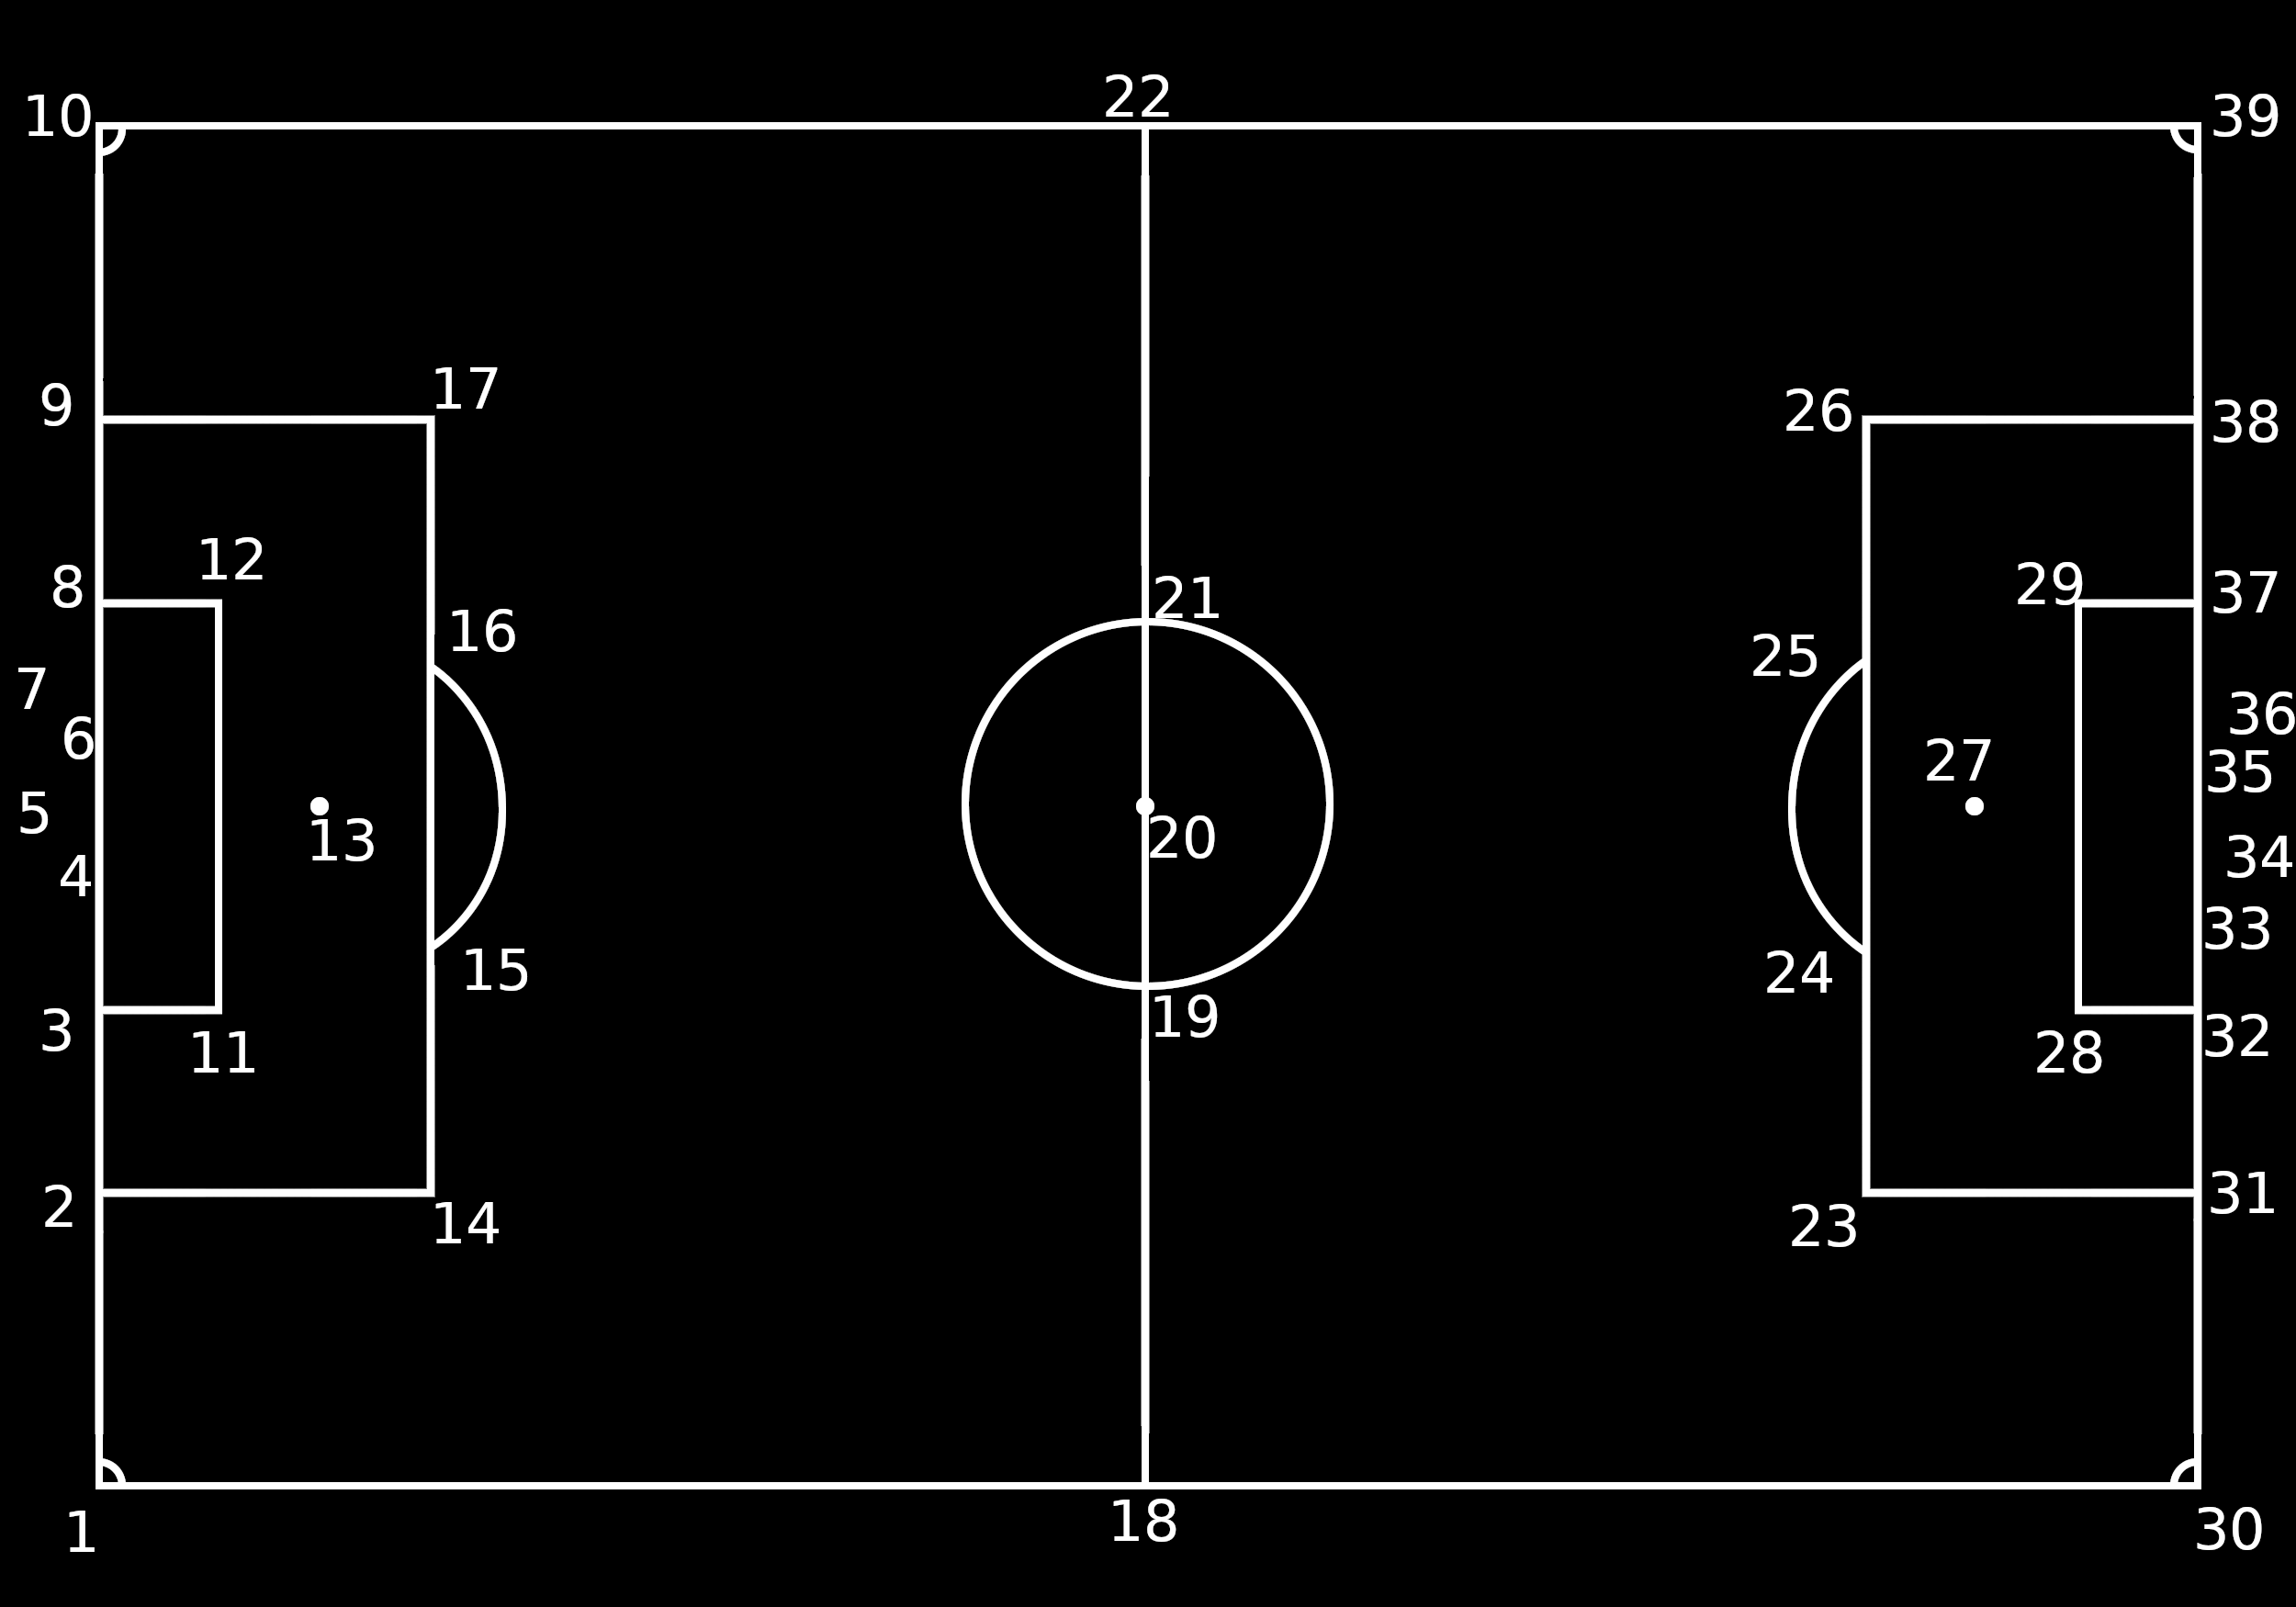
\includegraphics[keepaspectratio, width=\columnwidth]{coordinates.png}{text
    \caption{caption}
    \label{img:1}
\end{figure}
\ref{img:1} description} created 3d reference system that maps the points recognisable by the camera. This will be used for the artificial intelligence model to train the model and to process the video stream to perform the homographic transformation.

\begin{figure}[H]
    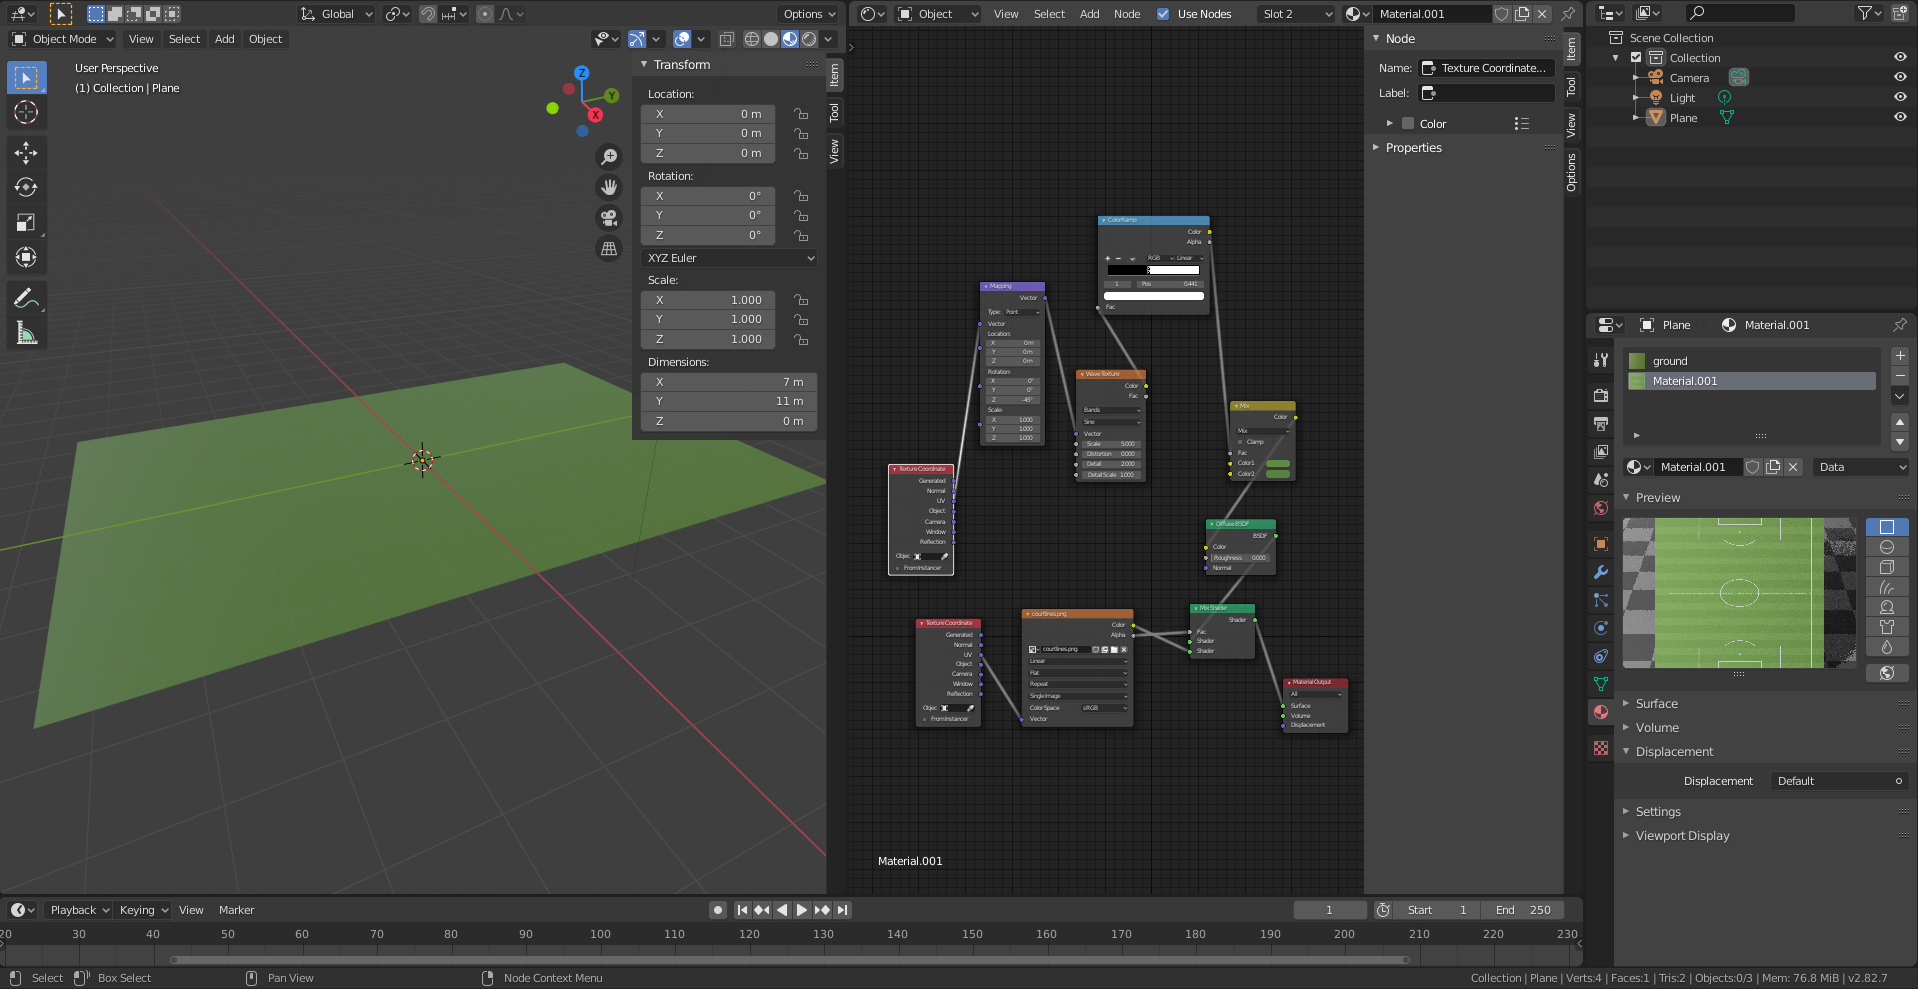
\includegraphics[keepaspectratio, width=\columnwidth]{Screenshot_from_2021-10-22_13-59-52.png}
    \caption{caption}
    \label{img:1}
\end{figure}
\ref{img:1} The 3d model was developed on blender. It is a green 3d texture (to emulate the grass) with a pitch png transparent graphic to produce the white lines.

\begin{figure}[H]
    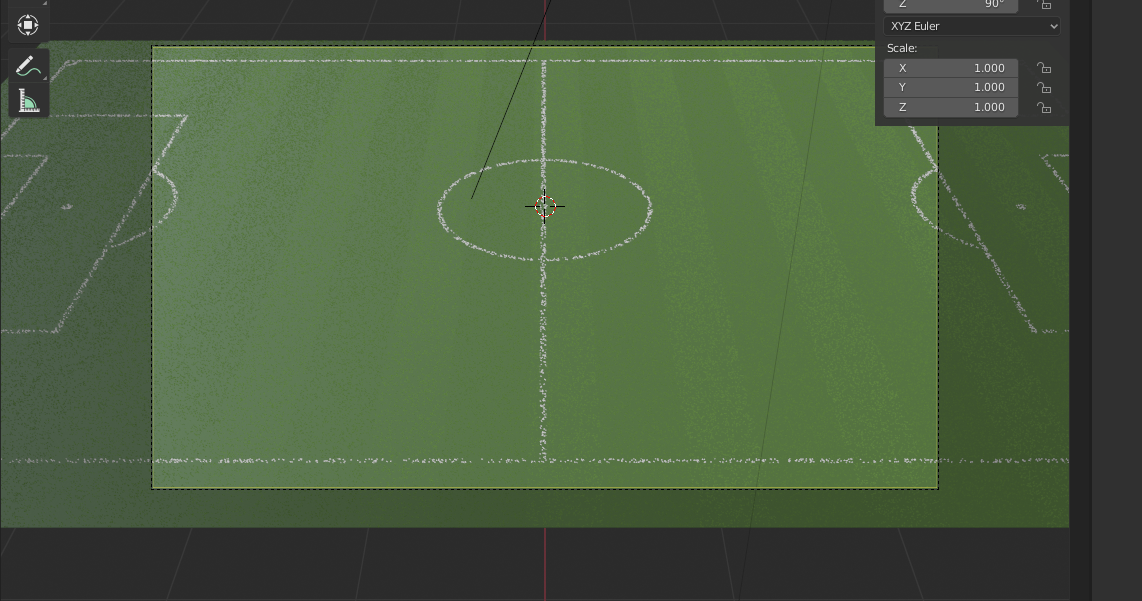
\includegraphics[keepaspectratio, width=\columnwidth]{Screenshot_2021-12-17_19-08-06.png}
    \caption{caption}
    \label{img:1}
\end{figure}
\ref{img:1} The result is a realistic pitch replica that can be rendered by a blender camera to produce the synthetic dataset


\begin{figure}[H]
    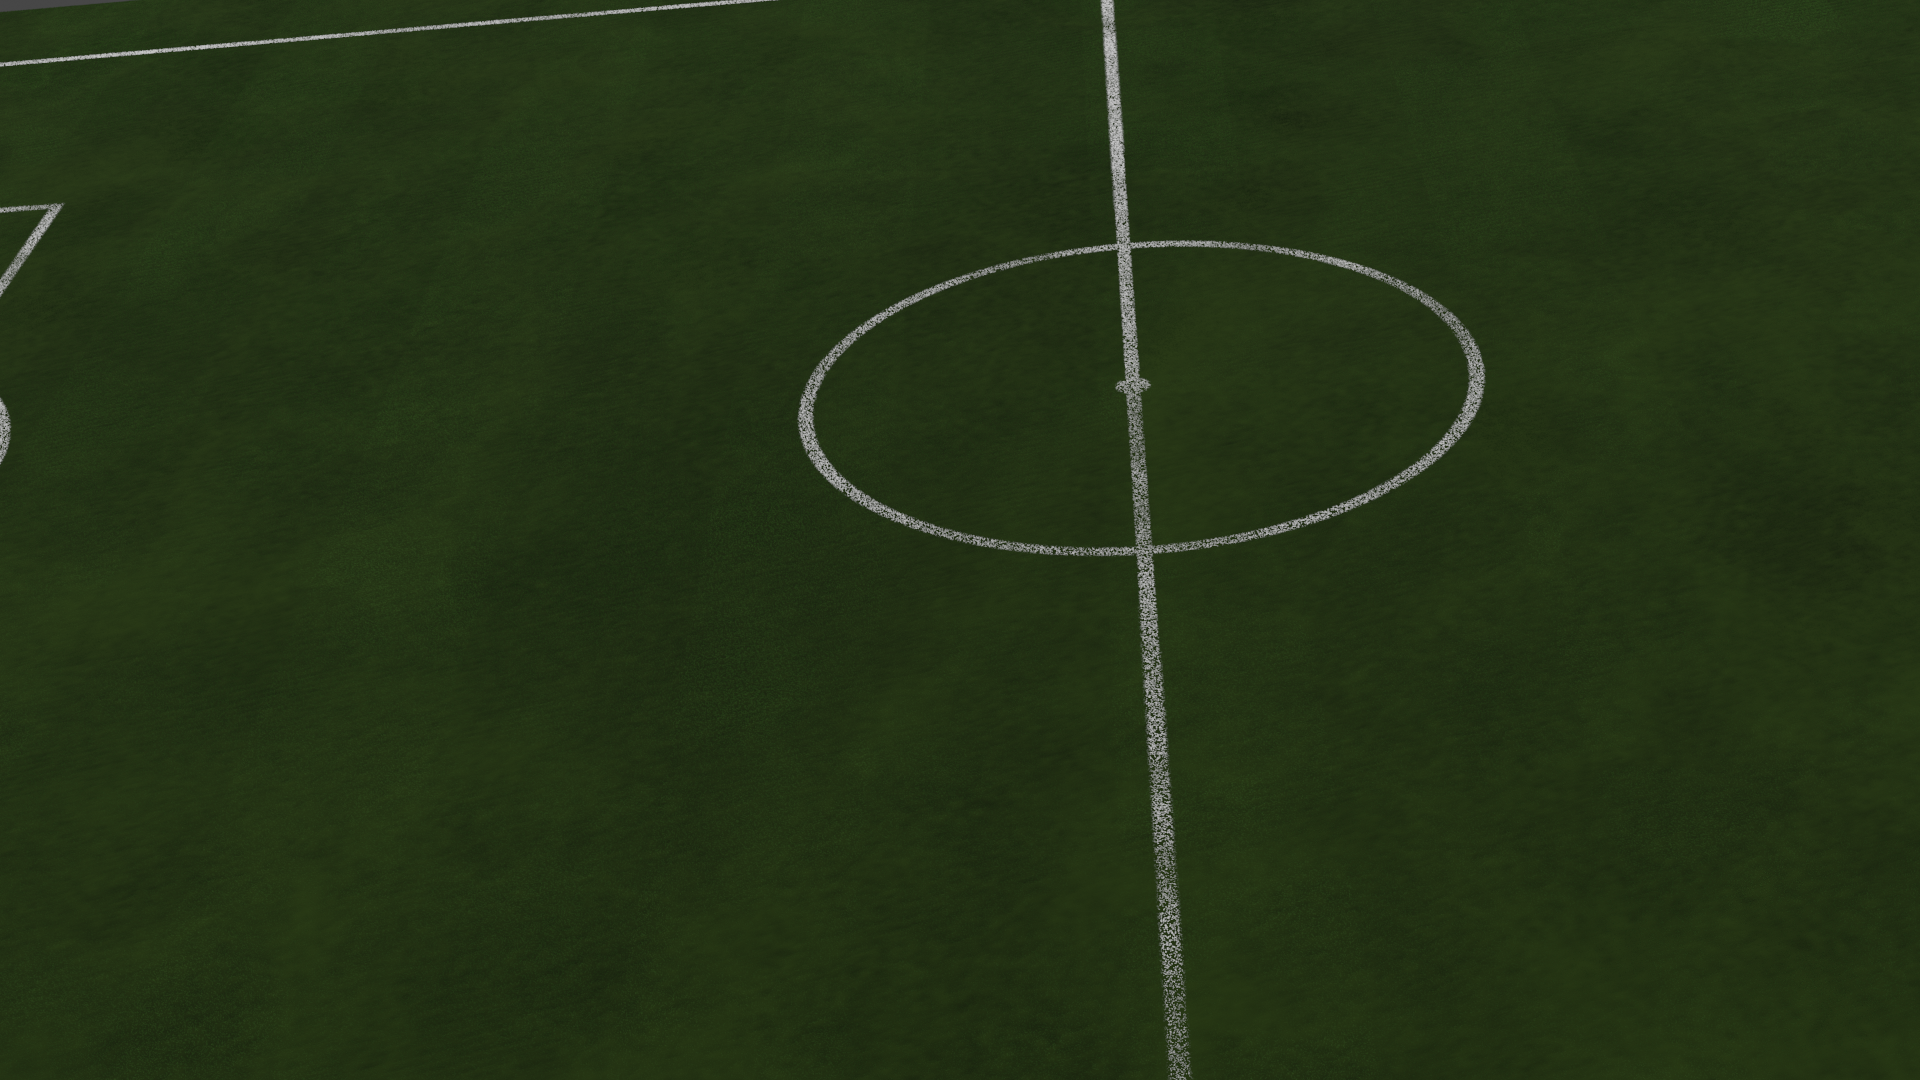
\includegraphics[keepaspectratio, width=\columnwidth]{image.png}
    \caption{caption}
    \label{img:1}
\end{figure}
\ref{img:1} this is the rendered image from a blender camera, this image is then the processed to be then used as the input for the artifical intelligence model.

\begin{figure}[H]
    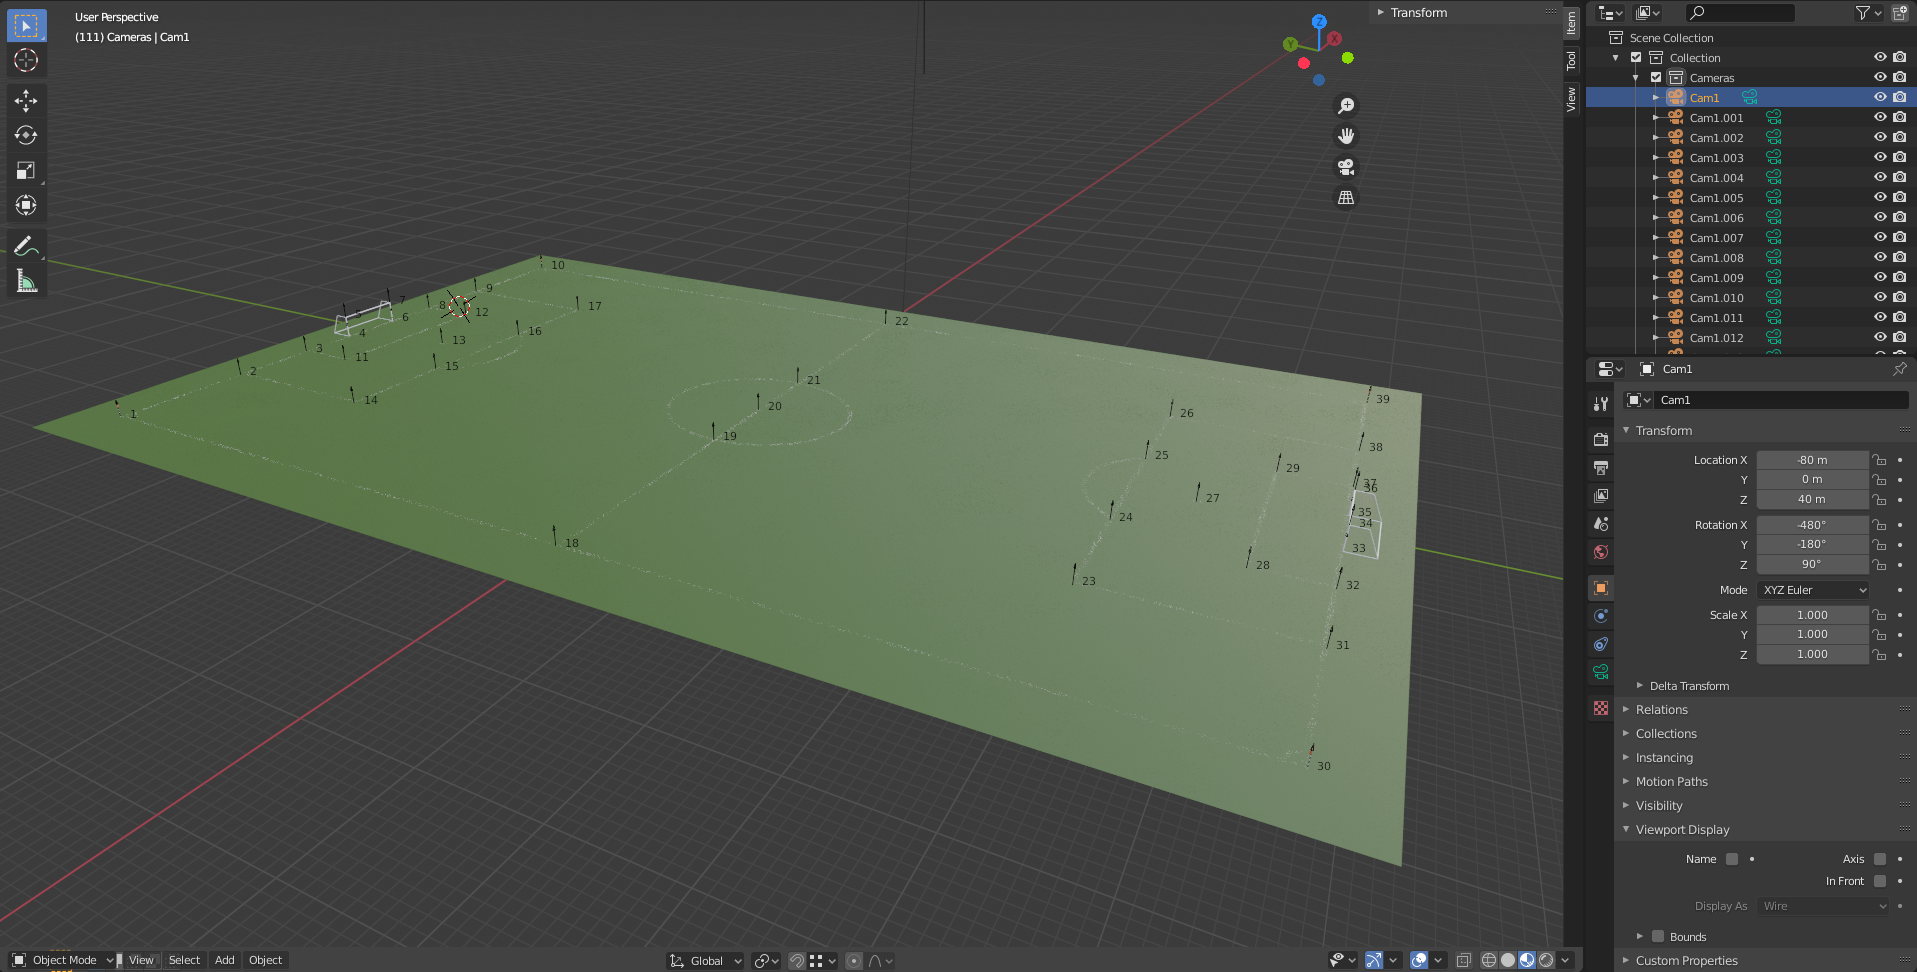
\includegraphics[keepaspectratio, width=\columnwidth]{Screenshot_2022-03-05_12-03-42.png}
    \caption{caption}
    \label{img:1}
\end{figure}
\ref{img:1} The pitch was then improved by adding 3d markers corresponding to the map reference system. These markers can be accessed by the blender cameras to retrieve their position on the camera view and their relative position to the cartesian origin.

\begin{figure}[H]
    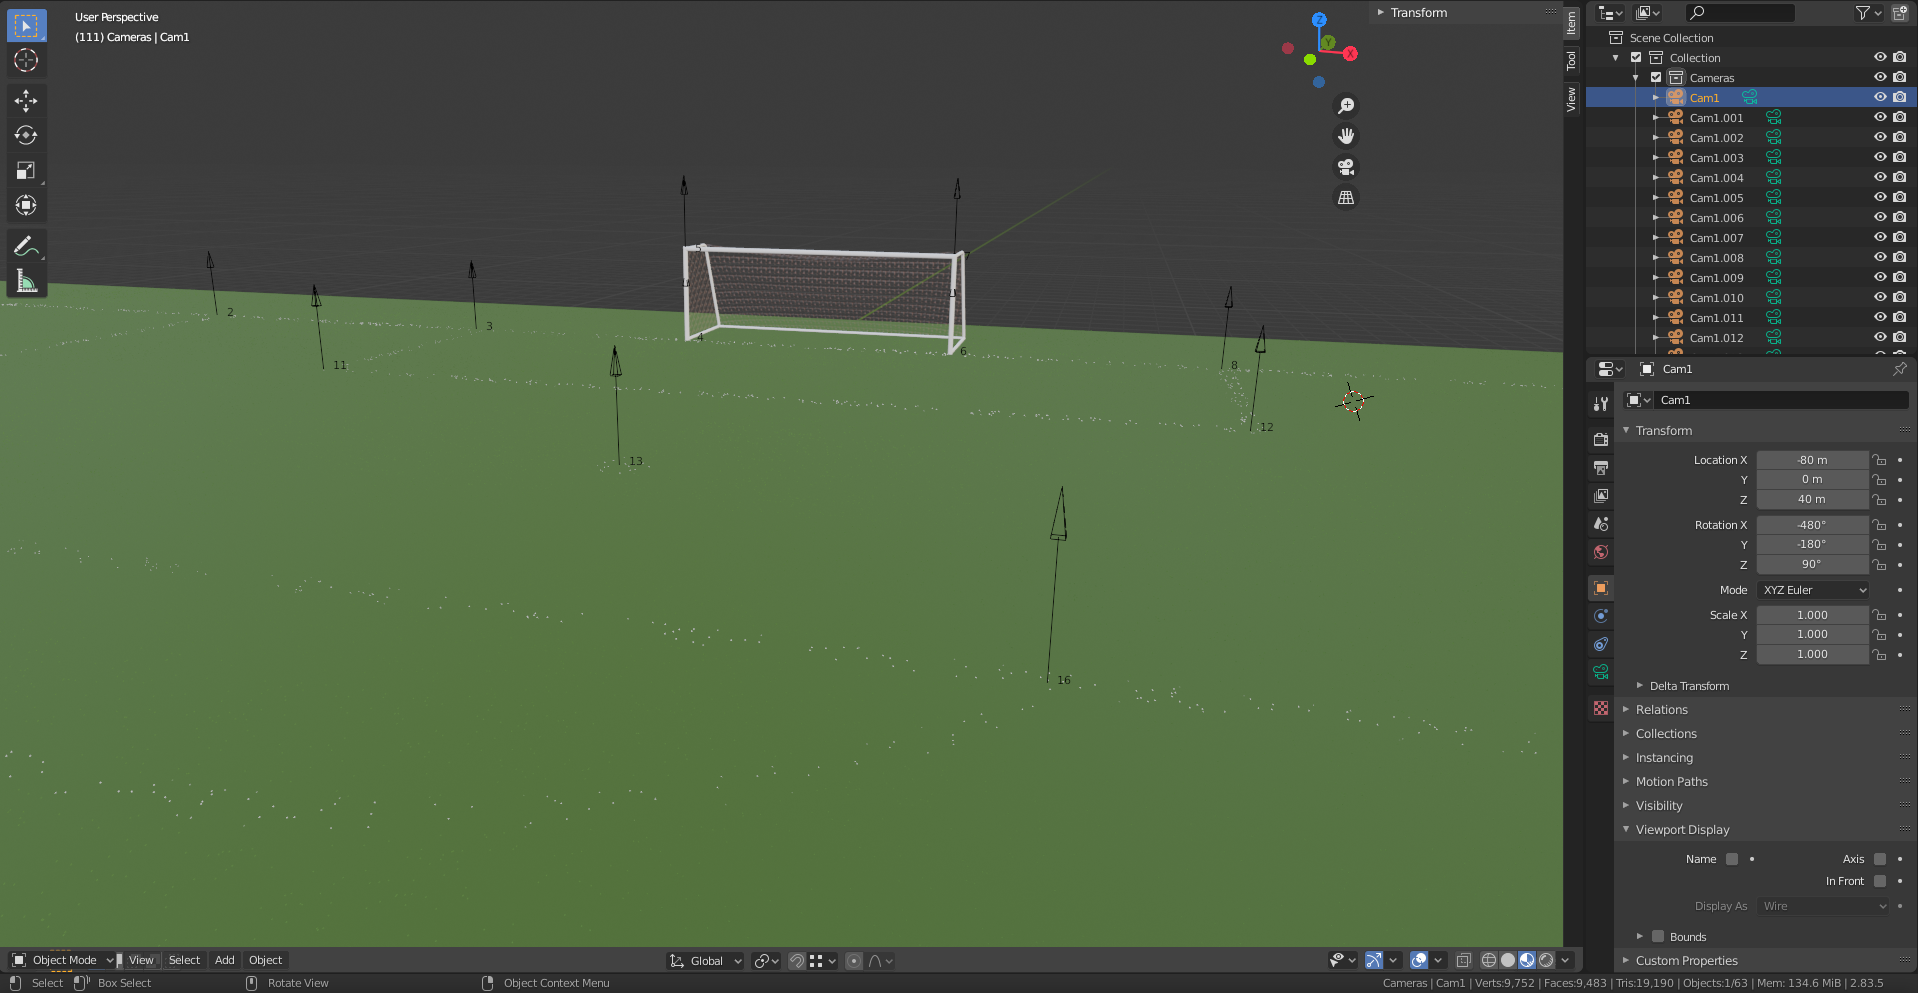
\includegraphics[keepaspectratio, width=\columnwidth]{Screenshot_2022-03-05_12-45-59.png}
    \caption{caption}
    \label{img:1}
\end{figure}
\ref{img:1} This is the view of the box which shows the position of the markers from a closer view

\begin{figure}[H]
    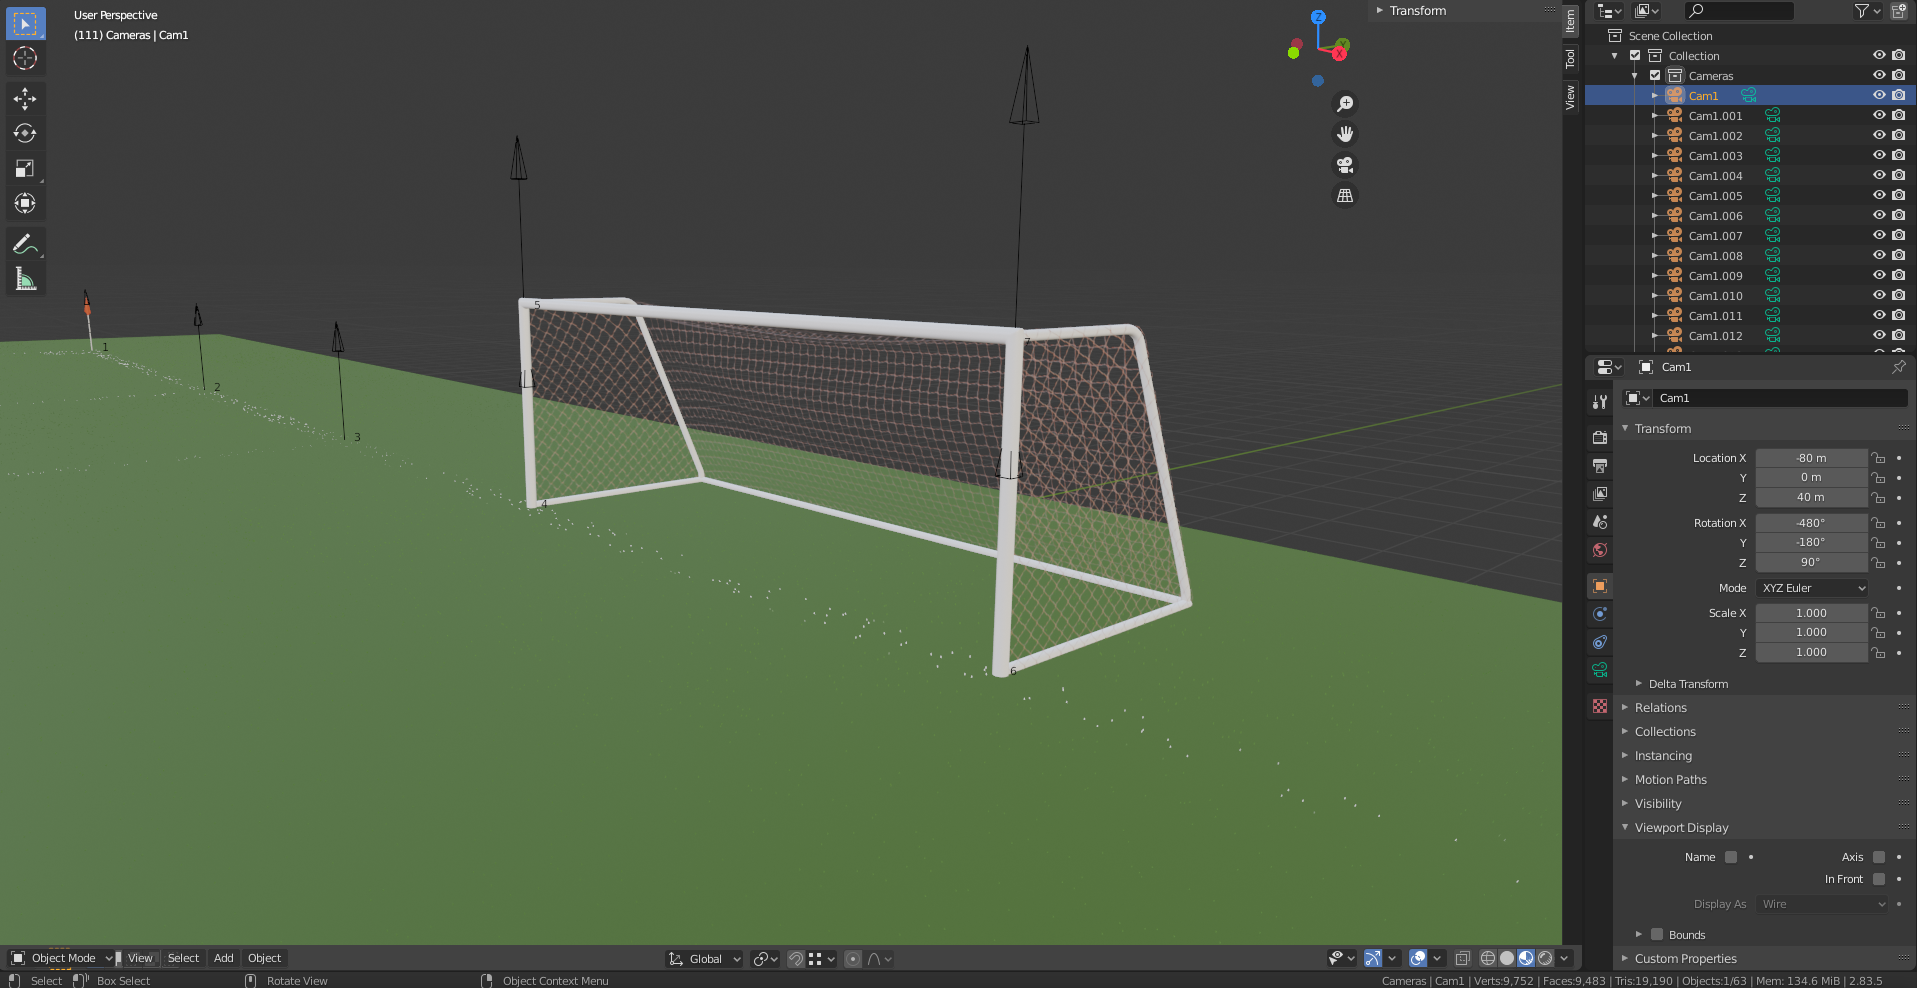
\includegraphics[keepaspectratio, width=\columnwidth]{Screenshot_2022-03-05_12-47-42.png}
    \caption{caption}
    \label{img:1}
\end{figure}
\ref{img:1} This is the view from the goal which is an important object that is important for image recognition. it has the only markers with a positive z-index to emulate the top corners of the goal. It also includes the corner flag (on the left) because all pitches have them by regulation.

\begin{figure}[H]
    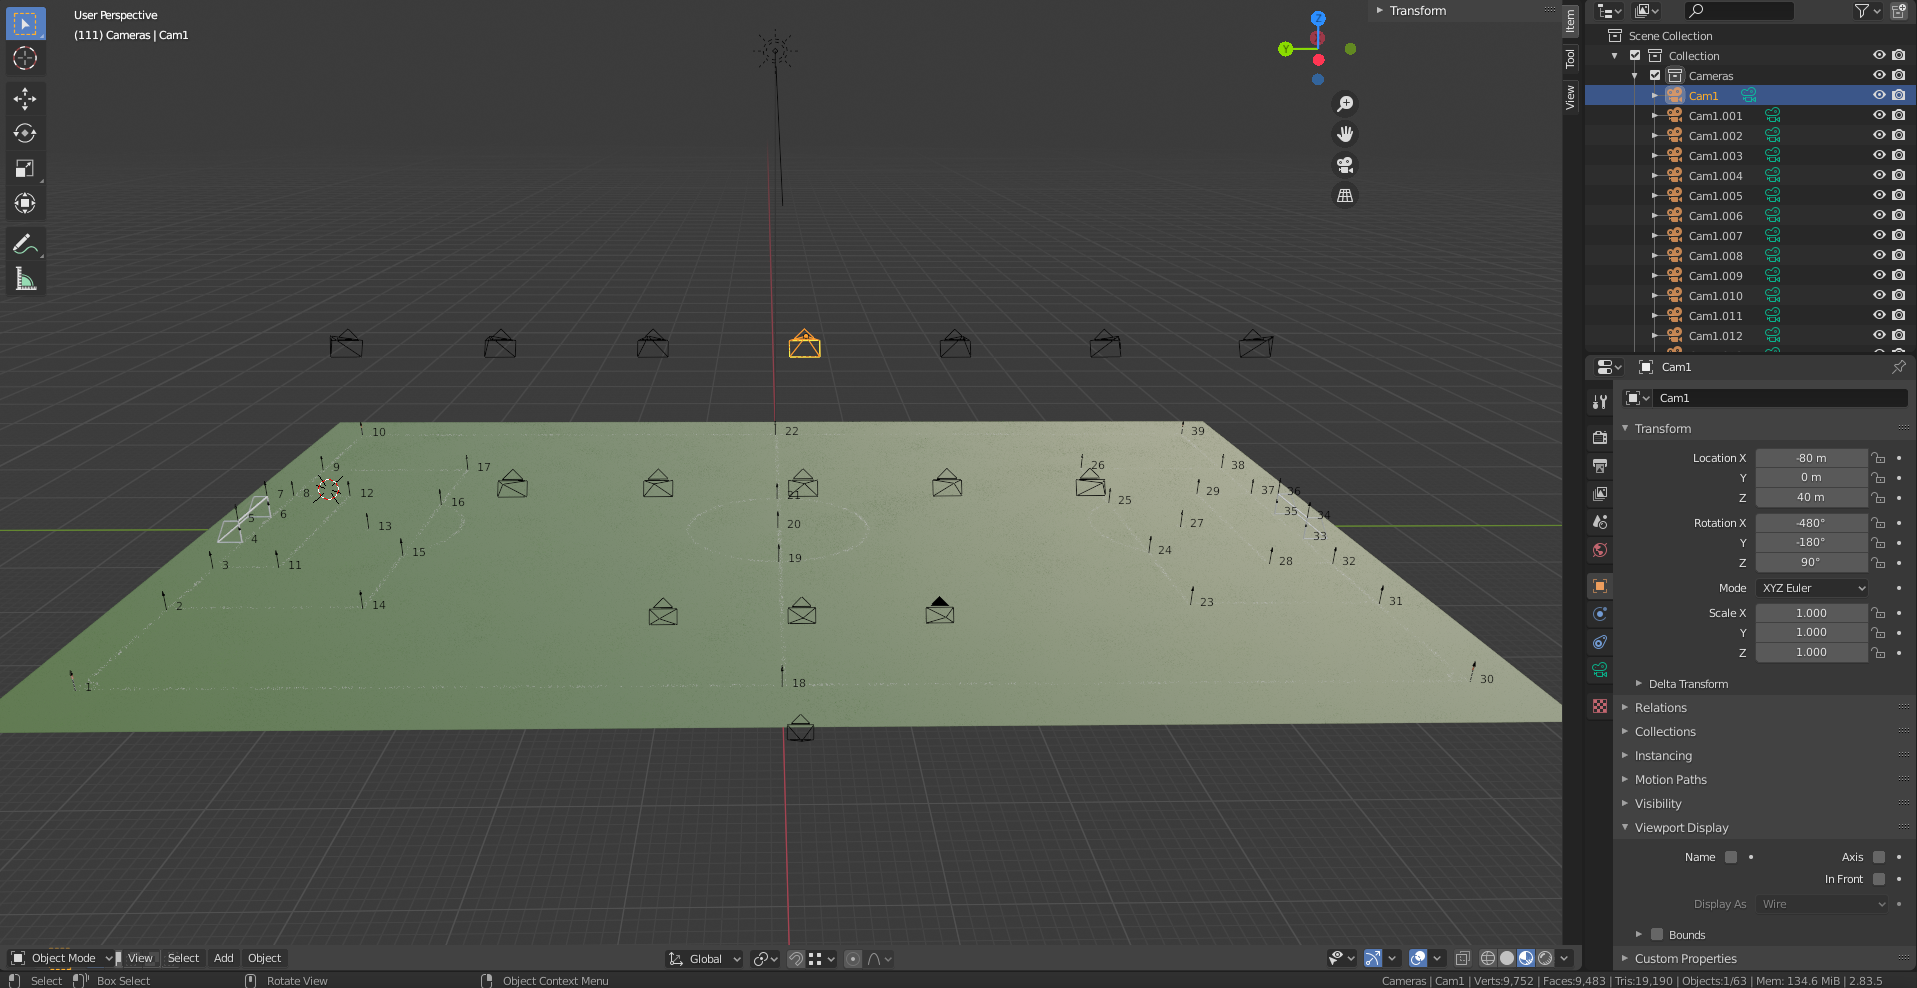
\includegraphics[keepaspectratio, width=\columnwidth]{Screenshot_2022-03-05_12-05-23.png}
    \caption{caption}
    \label{img:1}
\end{figure}
\ref{img:1} The final step is to create 15 cameras which will rotate within a range and will render images for the dataset from these different position to emulate the real camera which will be put in different positions.






\chapter{Testing}



\section{Testing assessment}

\begin{itemize}
\item
  testing with random camera, get accuracy
\item
  testing machine learning model accuracity over many layers

  \begin{itemize}
  \item
    configuration of convolution

    \begin{itemize}
    \item
      their kernels sizes
    \item
      number of filters
    \end{itemize}
  \item
    size of pool layers
  \item
    dropout rate
  \item
    number of flat dense layer when it has 2 inputs
  \end{itemize}
\end{itemize}



\section{Performance assessment}


text

\section{any other experimental work}


text

\chapter{Conclusions}



\section{main achievements}

    (relating them to initial objectives)
    (as well as similar worh from others)



\section{the main limitations of work}

\begin{itemize}
\item
  the output will always be an approximation (real world)
\item
  detect ball consistently
\item
  calculate ball trajectory
\item
  ball tracking is suspended whenever an object obstructs the camera
  view
\item
  players crossing eachother
\item
  cannot detect players outside camera frame. could create AI model for
  calculating probable player in position
\item
  cannot recognise players on camera frame. could create AI model for
  calculating their identity based on position/appearence
\item
  Currently not able to track 3d trajectory of objects
\item
  green masking may not work for non-green pitches and green kits
\end{itemize}



\section{possible extensions and future work}












\begin{itemize}
\item
  image/video processing operations (openCV)

  \begin{itemize}
  \item
    manual segmentation of video
  \item
    correction of ball labelling
  \item
    video/play segmentation
  \item
    detects "large human" (noise, needs to be removed), not removed until finding a neat algorithm, not priority for now
  \item
    recognise players

    \begin{itemize}
    \item
      identify players numbers
    \item
      identify players visual characteristics
    \end{itemize}
  \end{itemize}
\item
  dataset generation

  \begin{itemize}
  \item
    scale the blender model back to scale of 1, improve vector scaling function
  \item
      horizon problem, since some camera perspective may point to an infinite point, which is a problem( may put blender model in a box and check the intersection instead of infinite)
  \item
    add random noise to improve dataset and model
  \item
    video/play segmentation, maybe image clustering/unsopervised model to detect if it is repetition, different angle
  \end{itemize}
\item
  data collection

  \begin{itemize}
  \item
    spatio temporal data stream correction (pitch detection, player position detection, actions \ldots.)
  \item
    create data format (possibly logical ontology to leverage a logical reasoner) to create a richer dataset
  \item
    create algorithm to correct, smoth and fix data output stream
  \item
    collect event data
  \item
    collect tracking data
  \item
    synchronise event and tracking data
  \item
    synchronise footage and data timestamps

  \item
    space and spatial multiple image semantic matching
    \item
      is not real-time data collection algorithm
  \end{itemize}
\item
The greatest future improvement could be the integration of a 3d simulation environment which can be used to firstly enhance the current capabilities and additionally add extra functions that could take this project to the next level as a another source of synthetic data which could be complementary to the existing blender generation dataset environment. The Google Research Football Environment \ref{gfootball_env}, is a former open-source football computer game that was repurposed by Google's Artificial intelligence department to test and train AI adversary models in a highly stochastic environment. The project has been successful and it was used in many different AI events and competitions. It can be controlled by humans but the ultimate goal is to each team/players to be controlled by an intelligent agent in a realistic 3d physical environment that generates 3d positional data of all objects in the pitch. After training these models, the teams play against each other and generate important data that is used to evaluate the models performance. This final output data, along the corresponding visual data recorded, could be used to improve the training/validation/testing of the existing machine learning models for object and geometric detection models since the data collected intersects the one generated on blender. Although promissing, the real value is to use the in-game simulator to extract data that signals actions undertaken by players, 3d player pose estimation, objects 3d trajectory, in-game play segments and set piece recognition. These additional features are very valuable to increase the data points and enrich the data which contributes to automate ever more some manual operation that are performed by the operator. It is also concievable to create an extra model that corrects players tracking (to smoothing it out), and even augumenting the off-screen player positions (by combining spatio-temporal in-game data) which is trully groundbracking. Predicting the off-screen players position is critical because it mitigates one of the biggest limitations of this approach of using regular match-streams.
The Google Fooball environment \ref{gfootball_env} is specific to football what is contrary to objective of being a general solution for any sports. The long term solution in to create free- and open-source modular game environment to simulate other sports and even be used as bases for standalone sports games. This proposal is far fetched as it is a whole another project by itself but is is a sustainable project to leverage sports data science and gaming development. For these reasons this could be added to the community's long term roadmap.
\item
  methods will not apply this stage

  \begin{itemize}
  \item
    Human pose estimation
  \item
    3D human interaction
  \item
    Extrapolation; training against current data, to train and test action detection
  \item
    Object interaction tracking
  \item
    Multi-algorithm implementation (Detection -\textgreater{} tracking
    -\textgreater{} identification)
  \end{itemize}
\item
  general

  \begin{itemize}
  \item
    low quality footage
  \item
    weather and light visual conditions
  \item
    detect refs by colour
  \item
    accomodate differnt pitch colours
  \item
    ignoring people outside of the pitch
  \item
    short video (replay/sudden angles) segments interrupt data
    collection
    \item
     paralelise and multithread program
    \item
     move data generation and training to cloud.
    use of cloud computing instead of local machine
  \end{itemize}
\end{itemize}


\section{not implemented}

- not integrated the geometric reconstruction


\section{extra}

\begin{itemize}
\item
  when downloading copyrighted recordings or process data, reference
  source and its copyright
\item
  set up public dataset for public use by academics
\end{itemize}


\printbibliography


\end{document}
